\chapter{Vector Spaces}


\section{Vector Space}

\begin{enumerate}
    \item 
    \begin{definition}[Vector Space]
        A real-valued vector space $V = (\mathcal{V}, +, \cdot)$ is a set $\mathcal{V}$ with two operations:
        \hfill \cite{mfml/book/mml/Deisenroth-Faisal-Ong}
        \begin{enumerate}
            \item[] $+ :  \mathcal{V} \times \mathcal{V} \to \mathcal{V}$
            \hfill \cite{mfml/book/mml/Deisenroth-Faisal-Ong}
    
            \item[] $\cdot: \mathbb{R} \times \mathcal{V} \to \mathcal{V}$ 
            \hfill \cite{mfml/book/mml/Deisenroth-Faisal-Ong}
        \end{enumerate}
    \end{definition}


    \item addition ($+$) is inner operation: both operands must be from $\mathcal{V}$
    \hfill \cite{mfml/book/mml/Deisenroth-Faisal-Ong}

    \item multiplication by scalars ($\cdot$) is outer operation: one operand is from $\mathcal{V}$, another from $\mathbb{R}$
    \hfill \cite{mfml/book/mml/Deisenroth-Faisal-Ong}

    \item The elements $\bm{x} \in \mathcal{V}$ are called \textbf{vectors}.
    \hfill \cite{mfml/book/mml/Deisenroth-Faisal-Ong}
\end{enumerate}


\subsection{Properties of a vector Space}

\begin{enumerate}
    \item $(\mathcal{V}, +)$ is an Abelian group
    \hfill \cite{mfml/book/mml/Deisenroth-Faisal-Ong}

    \item Distributivity:
    \begin{enumerate}
        \item $\forall \lambda  \in  \mathbb{R}, \bm{x}, \bm{y} \in  \mathcal{V} : \lambda  \cdot  (\bm{x} + \bm{y}) = \lambda  \cdot  \bm{x} + \lambda  \cdot  \bm{y}$
        \hfill \cite{mfml/book/mml/Deisenroth-Faisal-Ong}

        \item $\forall \lambda , \psi  \in  \mathbb{R}, \bm{x} \in  \mathcal{V} : (\lambda  + \psi ) \cdot  \bm{x} = \lambda  \cdot  \bm{x} + \psi  \cdot  \bm{x}$
        \hfill \cite{mfml/book/mml/Deisenroth-Faisal-Ong}
    \end{enumerate}

    \item Associativity (outer operation): $\forall \lambda , \psi  \in  \mathbb{R}, \bm{x} \in  \mathcal{V} : \lambda \cdot (\psi \cdot x) = (\lambda \psi )\cdot \bm{x}$
    \hfill \cite{mfml/book/mml/Deisenroth-Faisal-Ong}

    \item Neutral element with respect to the outer operation: $\forall \bm{x} \in  \mathcal{V} : 1\cdot \bm{x} = \bm{x}$
    \hfill \cite{mfml/book/mml/Deisenroth-Faisal-Ong}

    \item The neutral element of $(\mathcal{V}, +)$ is the zero vector $\bm{0} = [0, \cdots , 0]^\top$
    \hfill \cite{mfml/book/mml/Deisenroth-Faisal-Ong}

    \item A “vector multiplication” $\bm{ab}, \bm{a}, \bm{b} \in \mathbb{R}^n$, is \textbf{not defined}.
    \hfill \cite{mfml/book/mml/Deisenroth-Faisal-Ong}
\end{enumerate}


\subsection{Dimension of a vector Space}


\begin{enumerate}
    \item the dimension of $V$ is the number of basis vectors of $V$ , and we write $\dim(V)$.
    \hfill \cite{mfml/book/mml/Deisenroth-Faisal-Ong}

    \item The dimension of a vector space corresponds to the number of its basis vectors.
    \hfill \cite{mfml/book/mml/Deisenroth-Faisal-Ong}

    \item Intuitively, the dimension of a vector space can be thought of as the number of independent directions in this vector space.
    \hfill \cite{mfml/book/mml/Deisenroth-Faisal-Ong}

    \item The dimension of a vector space is not necessarily the number of elements in a vector. 
    For instance, the vector space $V = \text{span}[\begin{bmatrix}0 \\ 1\end{bmatrix}]$ is one-dimensional, although the basis vector possesses two elements.
    \hfill \cite{mfml/book/mml/Deisenroth-Faisal-Ong}
\end{enumerate}


\begin{lstlisting}[
    language=Python,
    caption=Dimension of vector space - numPy
]
import numpy as np

# Define 3 column vectors in R^4
v1 = np.array([1, 2, 3, 4]).reshape(-1, 1)
v2 = np.array([2, 4, 6, 8]).reshape(-1, 1)
v3 = np.array([0, 1, 0, 1]).reshape(-1, 1)

# Put them into a matrix as columns => stack column-wise (axis=1)
matrix = np.column_stack([v1, v2, v3])  # Shape: (4, 3)

# Find the dimension = rank of the matrix
dimension = np.linalg.matrix_rank(matrix)

print(f"Dimension of the vector space: {dimension}")
\end{lstlisting}












\subsection{Norm}

\begin{enumerate}
    \item 
    \begin{definition}[Norm]
        A norm on a vector space $V$ is a function
        \hfill \cite{mfml/book/mml/Deisenroth-Faisal-Ong}
        \\
        .\hfill
        $\dnorm{\cdot}: V \to \mathbb{R}$ such that $\bm{x} \mapsto \dnorm{\bm{x}}$
        \hfill \cite{mfml/book/mml/Deisenroth-Faisal-Ong}
        \\
        which assigns each vector $\bm{x}$ its length $\dnorm{\bm{x}} \in \mathbb{R}$, such that for all $\lambda \in \mathbb{R}$ and $\bm{x}, \bm{y} \in V$ the following hold:
        \hfill \cite{mfml/book/mml/Deisenroth-Faisal-Ong}
    \end{definition}
    \begin{enumerate}
        \item Absolutely homogeneous: $\dnorm{\lambda \bm{x}} = \dabs{\lambda} \dnorm{\bm{x}}$
        \hfill \cite{mfml/book/mml/Deisenroth-Faisal-Ong}

        \item Triangle inequality: $\dnorm{\bm{x} + \bm{y}} \leq \dnorm{\bm{x}} + \dnorm{\bm{y}}$
        \hfill \cite{mfml/book/mml/Deisenroth-Faisal-Ong}
        \\
        In geometric terms, the triangle inequality states that for any triangle, the sum of the lengths of any two sides must be greater than or equal to the length of the remaining side.
        \hfill \cite{mfml/book/mml/Deisenroth-Faisal-Ong}

        \item Positive definite: $\dnorm{\bm{x}} \geq 0$ and $\dnorm{\bm{x}} = 0 \Longleftrightarrow \bm{x} = \bm{0}$
        \hfill \cite{mfml/book/mml/Deisenroth-Faisal-Ong}
    \end{enumerate}
\end{enumerate}




\begin{lstlisting}[
    language=Python,
    caption=General Norm of a vector - numPy
]
import numpy as np

def norm_general(_arr: np.ndarray):
    """
    Compute the norm using custom formula/ calculations
    """
    raise NotImplementedError()
\end{lstlisting}






\subsection{General Inner Product ( $\Omega(a, b)$ )}

\begin{enumerate}
    \item A bilinear mapping $\Omega$ is a mapping with two arguments, and it is linear in each argument, i.e., when we look at a vector space $V$ then it holds that for all $\bm{x}, \bm{y}, \bm{z} \in V, \lambda , \psi  \in \mathbb{R}$ that
    \hfill \cite{mfml/book/mml/Deisenroth-Faisal-Ong}
    \\
    .\hfill
    $\Omega(\lambda \bm{x} + \psi \bm{y}, \bm{z}) = \lambda \Omega(\bm{x}, \bm{z}) + \psi \Omega(\bm{y}, \bm{z})$
    \hfill \cite{mfml/book/mml/Deisenroth-Faisal-Ong}
    \\
    .\hfill
    $\Omega(\bm{x}, \lambda \bm{y} + \psi \bm{z}) = \lambda \Omega(\bm{x}, \bm{y}) + \psi \Omega(\bm{x}, \bm{z})$.
    \hfill \cite{mfml/book/mml/Deisenroth-Faisal-Ong}

    \item Let $V$ be a vector space and $\Omega : V \times  V \to \mathbb{R}$ be a bilinear mapping that takes two vectors and maps them onto a real number. Then
    \hfill \cite{mfml/book/mml/Deisenroth-Faisal-Ong}
    \begin{enumerate}
        \item $\Omega$ is called \textbf{symmetric} if $\Omega(\bm{x}, \bm{y}) = \Omega(\bm{y}, \bm{x})$ for all $\bm{x}, \bm{y} \in  V$ , i.e., the order of the arguments does not matter.
        \hfill \cite{mfml/book/mml/Deisenroth-Faisal-Ong}

        \item $\Omega$ is called \textbf{positive definite} if $\forall \bm{x} \in  V \backslash \dCurlyBrac{\bm{0}} : \Omega(\bm{x}, \bm{x}) > 0 , \Omega(\bm{0}, \bm{0}) = 0$.
        \hfill \cite{mfml/book/mml/Deisenroth-Faisal-Ong}
    \end{enumerate}

\end{enumerate}





\subsection{Inner Product ( $<x, y>$ )}

\begin{enumerate}
    \item Let $V$ be a vector space and $\Omega  : V \times  V \to  \mathbb{R}$ be a bilinear mapping that takes two vectors and maps them onto a real number. Then
    \hfill \cite{mfml/book/mml/Deisenroth-Faisal-Ong}
    \begin{enumerate}
        \item A positive definite, symmetric bilinear mapping $\Omega  : V \times  V \to  \mathbb{R}$ is called an inner product on $V$ . 
        We typically write $\dAngleBrac{x, y}$ instead of $\Omega (x, y)$.        
        \hfill \cite{mfml/book/mml/Deisenroth-Faisal-Ong}
    \end{enumerate}

    \item default inner product is dot product: $\dAngleBrac{\bm{x}, \bm{y}} = \bm{x}^\top \bm{y}$
    \hfill \cite{mfml/book/mml/Deisenroth-Faisal-Ong}
\end{enumerate}







\subsection{Inner Product Space}

\begin{enumerate}
    \item Let $V$ be a vector space and $\Omega  : V \times  V \to  \mathbb{R}$ be a bilinear mapping that takes two vectors and maps them onto a real number. 
    Then the pair $(V, \dAngleBrac{\cdot, \cdot})$ is called an \textbf{inner product space} or \textbf{(real) vector space with inner product}.
\end{enumerate}




\subsection{Euclidean vector space}

\begin{enumerate}
    \item Let $V$ be a vector space and $\Omega : V \times V \to \mathbb{R}$ be a bilinear mapping that takes two vectors and maps them onto a real number. Then if we use the dot product, we call $(V,\dAngleBrac{\cdot, \cdot})$ a Euclidean vector space.
\end{enumerate}



\subsection{Lengths}

\begin{enumerate}
    \item Inner products and norms are closely related in the sense that any inner product induces a norm
    \hfill \cite{mfml/book/mml/Deisenroth-Faisal-Ong}
    \\
    .\hfill
    $\dnorm{\bm{x}} := \sqrt{\dAngleBrac{\bm{x}, \bm{x}}}$
    \hfill \cite{mfml/book/mml/Deisenroth-Faisal-Ong}
    \\
    in a natural way, such that we can compute lengths of vectors using the inner product.
    \hfill \cite{mfml/book/mml/Deisenroth-Faisal-Ong}

    \item length depends on norm
    \hfill \cite{common/online/chatgpt}
    \\
    different norms lead to different lengths
    \hfill \cite{common/online/chatgpt}

    \item Not every norm is induced by an inner product (eg: Manhattan norm).
    \hfill \cite{mfml/book/mml/Deisenroth-Faisal-Ong}

    \item 
    \begin{definition}[Cauchy-Schwarz Inequality]
    For an inner product vector space $(V,\dAngleBrac{\cdot, \cdot})$ the induced norm $\dnorm{\cdot}$ satisfies the Cauchy-Schwarz inequality
    \hfill \cite{mfml/book/mml/Deisenroth-Faisal-Ong}
    \\
    .\hfill
    $\dabs{\dAngleBrac{\bm{x}, \bm{y}}} \leq \dnorm{\bm{x}} \dnorm{\bm{y}}$
    \hfill \cite{mfml/book/mml/Deisenroth-Faisal-Ong}
    \end{definition}

    \item Transformations by orthogonal matrices are special because the length of a vector $\bm{x}$ is not changed when transforming it using an orthogonal matrix $\bm{A}$. 
    For the dot product, we obtain
    \hfill \cite{mfml/book/mml/Deisenroth-Faisal-Ong}
    \\
    .\hfill
    $
        \dnorm{\bm{Ax}}^2 
        = (\bm{Ax})^\top (\bm{Ax})
        = \bm{x}^\top \bm{A}^\top \bm{Ax}
        = \bm{x}^\top \bm{Ix}
        = \bm{x}^\top \bm{x}
        = \dnorm{\bm{x}}^2
    $
    \hfill \cite{mfml/book/mml/Deisenroth-Faisal-Ong}
\end{enumerate}





\subsection{Distance}

\begin{enumerate}
    \item Consider an inner product space $(V,\dAngleBrac{\cdot, \cdot})$. 
    Then
    \hfill \cite{mfml/book/mml/Deisenroth-Faisal-Ong}
    \\
    .\hfill
    $
        d(\bm{x}, \bm{y})
        := \dnorm{\bm{x} - \bm{y}}
        = \sqrt{\dAngleBrac{\bm{x} - \bm{y}, \bm{x} - \bm{y}}}
    $
    \hfill \cite{mfml/book/mml/Deisenroth-Faisal-Ong}
    \\
    is called the distance between $\bm{x}$ and $\bm{y}$ for $\bm{x}, \bm{y} \in V$ .
    \hfill \cite{mfml/book/mml/Deisenroth-Faisal-Ong}

    \item If we use the dot product as the inner product, then the distance is called \textbf{Euclidean distance}.
    \hfill \cite{mfml/book/mml/Deisenroth-Faisal-Ong}

    \item Similar to the length of a vector, the distance between vectors does not require an inner product: a norm is sufficient.
    If we have a norm induced by an inner product, the distance may vary depending on the choice of the inner product. 
    \hfill \cite{mfml/book/mml/Deisenroth-Faisal-Ong}

    \item Every distance is a metric, but not every metric is necessarily defined as a distance using a norm or inner product.
    \hfill \cite{common/online/chatgpt}

    \item Transformations with orthogonal matrices preserve distances.
    \hfill \cite{mfml/book/mml/Deisenroth-Faisal-Ong}
\end{enumerate}




\subsection{Metric}

\begin{enumerate}
    \item 
    \begin{definition}[Metric]
        The mapping $d : V \times V \to \mathbb{R}$, $(\bm{x}, \bm{y}) \mapsto d(\bm{x}, \bm{y})$ is called a \textbf{metric}.
        \hfill \cite{mfml/book/mml/Deisenroth-Faisal-Ong}
    \end{definition}

    \item A metric $d$ satisfies the following:
    \hfill \cite{mfml/book/mml/Deisenroth-Faisal-Ong}
    \begin{enumerate}
        \item $d$ is \textbf{positive definite}, i.e., $d(\bm{x}, \bm{y}) \geq 0$ for all $\bm{x}, \bm{y} \in V$ and $d(\bm{x}, \bm{y}) = 0 \Longleftrightarrow \bm{x} = \bm{y}$ .
        \hfill \cite{mfml/book/mml/Deisenroth-Faisal-Ong}

        \item $d$ is \textbf{symmetric}, i.e., $d(\bm{x}, \bm{y}) = d(\bm{y}, \bm{x})$ for all $\bm{x}, \bm{y} \in V$ .
        \hfill \cite{mfml/book/mml/Deisenroth-Faisal-Ong}

        \item \textbf{Triangle inequality}: $d(\bm{x}, \bm{z}) \leq d(\bm{x}, \bm{y}) + d(\bm{y}, \bm{z})$ for all $\bm{x}, \bm{y}, \bm{z} \in V$ .
        \hfill \cite{mfml/book/mml/Deisenroth-Faisal-Ong}
    \end{enumerate}
\end{enumerate}



\subsection{Inner Product VS Metric}

\begin{enumerate}
    \item the lists of properties of inner products and metrics look very similar. 
    \hfill \cite{mfml/book/mml/Deisenroth-Faisal-Ong}

    \item $\dAngleBrac{\bm{x}, \bm{y}}$ and $d(\bm{x}, \bm{y})$ behave in opposite directions.
    \hfill \cite{mfml/book/mml/Deisenroth-Faisal-Ong}

    \item Very similar $\bm{x}$ and $\bm{y}$ will result in a large value for the inner product and a small value for the metric.
    \hfill \cite{mfml/book/mml/Deisenroth-Faisal-Ong}
\end{enumerate}




\subsection{Angles}

\begin{enumerate}
    \item We use the Cauchy-Schwarz inequality to define angles $\omega$ in inner product spaces between two vectors $\bm{x}, \bm{y}$, and this notion coincides with our intuition in $\mathbb{R}^2$ and $\mathbb{R}^3$. 
    Assume that $\bm{x} \neq \bm{0}$, $\bm{y} \neq \bm{0}$. 
    Then
    $
        -1 \leq \dfrac{\dAngleBrac{\bm{x}, \bm{y}}}{\dnorm{\bm{x}} \dnorm{\bm{y}}} \leq 1
    $. 
    Therefore, there exists a unique $\omega \in [0, \pi]$ with 
    $
        \cos(\omega) = \dfrac{\dAngleBrac{\bm{x}, \bm{y}}}{\dnorm{\bm{x}} \dnorm{\bm{y}}}
    $
    \hfill \cite{mfml/book/mml/Deisenroth-Faisal-Ong}

    \item The number $\omega$ is the angle between the vectors $\bm{x}$ and $\bm{y}$.
    \hfill \cite{mfml/book/mml/Deisenroth-Faisal-Ong}

    \item Intuitively, the angle between two vectors tells us how similar their orientations are.
    \hfill \cite{mfml/book/mml/Deisenroth-Faisal-Ong}

    \item Transformations with orthogonal matrices preserve angles.
    \hfill \cite{mfml/book/mml/Deisenroth-Faisal-Ong}
    \\
    The angle between any two vectors $\bm{x}, \bm{y}$, as measured by their inner product, is also unchanged when transforming both of them using an orthogonal matrix $\bm{A}$. 
    Assuming the dot product as the inner product, the angle of the images $\bm{Ax}$ and $\bm{Ay}$ is given as
    \hfill \cite{mfml/book/mml/Deisenroth-Faisal-Ong}
    \\
    .\hfill
    $
        \cos \omega
        = \dfrac{(\bm{Ax})^\top (\bm{Ax})}{\dnorm{\bm{Ax}} \dnorm{\bm{Ax}}}
        = \dfrac{\bm{x}^\top \bm{A}^\top\bm{Ay}}{\sqrt{\bm{x}^\top \bm{A}^\top\bm{Ax} \bm{y}^\top \bm{A}^\top\bm{Ay}}}
        = \dfrac{\bm{x}^\top \bm{y}}{\dnorm{\bm{x}} \dnorm{\bm{y}}}
    $
    \hfill \cite{mfml/book/mml/Deisenroth-Faisal-Ong}
    \\
    which gives exactly the angle between $\bm{x}$ and $\bm{y}$.
\end{enumerate}

\begin{customArrayStretch}{1.3}
\begin{table}[H]
    \centering
    \begin{tabular}{|l|l|l|}
        \hline
        $\omega$ & $\cos(\omega)$ & Interpretation \\
        \hline
        $0$ & $1$ & orientation is same \\
        ${\pi}/{2}$ & $0$ & perpendicular \\
        $\pi$ & $-1$ & opposite direction \\
        \hline
    \end{tabular}
\end{table}
\end{customArrayStretch}







\subsection{Orthogonal Complement ( $U^\perp$ )}

\begin{enumerate}
    \item Consider a $D$-dimensional vector space $V$ and an $M$-dimensional subspace $U \subseteq V$ . 
    Then its orthogonal complement $U^\perp$ is a $(D-M)$-dimensional subspace of $V$ and contains all vectors in $V$ that are orthogonal to every vector in $U$. 
    Furthermore, $U \cap U^\perp = \dCurlyBrac{\bm{0}}$ so that any vector $\bm{x} \in V$ can be uniquely decomposed into
    \hfill \cite{mfml/book/mml/Deisenroth-Faisal-Ong}
    \\
    .\hfill
    $
        \bm{x}
        = \dsum^M_{m=1} \lambda_m \bm{b}_m + \dsum ^{D-M}_{j=1} \psi_j \bm{b}_j^\perp
        \hspace{1cm}
        \lambda_m, \psi_j \in \mathbb{R}
    $
    \hfill \cite{mfml/book/mml/Deisenroth-Faisal-Ong}
    \\
    where $(\bm{b}_1, \cdots , \bm{b}_M)$ is a basis of $U$ and $(\bm{b}^\perp _1 , \cdots , \bm{b}^\perp _{D-M})$ is a basis of $U^\perp$.
    \hfill \cite{mfml/book/mml/Deisenroth-Faisal-Ong}

    \item the orthogonal complement can also be used to describe a plane $U$ (two-dimensional subspace) in a three-dimensional vector space.
    \hfill \cite{mfml/book/mml/Deisenroth-Faisal-Ong}

    \item the vector $\bm{w}$ with $\dnorm{\bm{w}} = 1$, which is orthogonal to the plane $U$, is the basis vector of $U^\perp$.
    All vectors that are orthogonal to $\bm{w}$ must (by construction) lie in the plane $U$. 
    The vector $\bm{w}$ is called the \textbf{normal vector} of $U$.
    \hfill \cite{mfml/book/mml/Deisenroth-Faisal-Ong}

    \item orthogonal complements can be used to describe hyperplanes in $n$-dimensional vector and affine spaces.
    \hfill \cite{mfml/book/mml/Deisenroth-Faisal-Ong}
\end{enumerate}




































\section{Vector Subspace/ linear subspace}


\begin{enumerate}
    \item 
    \begin{definition}[Vector Subspace]
        Let $V = (\mathcal{V}, +, \cdot )$ be a vector space and $\mathcal{U} \subseteq \mathcal{V}, \mathcal{U} \neq \phi$. 
        Then $U = (\mathcal{U}, +, \cdot )$ is called vector subspace of $V$ (or linear subspace) if $U$ is a vector space with the vector space operations $+$ and $\cdot$  restricted to $\mathcal{U} \times \mathcal{U}$ and $\mathbb{R} \times \mathcal{U}$. 
        We write $U \subseteq V$ to denote a subspace $U$ of $V$.
        \hfill \cite{mfml/book/mml/Deisenroth-Faisal-Ong}
    \end{definition}

    \item Intuitively, they are sets contained in the original vector space with the property that when we perform vector space operations on elements within this subspace, we will never leave it. 
    In this sense, they are “closed”.
    \hfill \cite{mfml/book/mml/Deisenroth-Faisal-Ong}

    \item If $\mathcal{U} \subseteq \mathcal{V}$ and $V$ is a vector space, then $U$ naturally inherits many properties directly from $V$ because they hold for all $\bm{x} \in \mathcal{V}$, and in particular for all $\bm{x} \in \mathcal{U} \subseteq \mathcal{V}$. 
    This includes the Abelian group properties, the distributivity, the associativity and the neutral element.
    \hfill \cite{mfml/book/mml/Deisenroth-Faisal-Ong}

    \item To determine whether $(\mathcal{U}, +, \cdot)$ is a subspace of V we still do need to show:
    \begin{enumerate}
        \item $\mathcal{U} \neq \phi$, in particular: $\bm{0} \in \mathcal{U}$
        \hfill \cite{mfml/book/mml/Deisenroth-Faisal-Ong}

        \item Closure of $U$:
        \begin{enumerate}
            \item With respect to the outer operation: $\forall \lambda  \in  \mathbb{R} \forall \bm{x} \in  \mathcal{U} : \lambda \bm{x} \in  \mathcal{U}$.
            \hfill \cite{mfml/book/mml/Deisenroth-Faisal-Ong}
            
            \item With respect to the inner operation: $\forall \bm{x}, \bm{y} \in  \mathcal{U} : \bm{x} + \bm{y} \in  \mathcal{U}$.
            \hfill \cite{mfml/book/mml/Deisenroth-Faisal-Ong}
        \end{enumerate}
    \end{enumerate}

\end{enumerate}


\subsection{Dimension of a Vector Subspace}

\begin{enumerate}
    \item If $U \subseteq V$ is a subspace of $V$ , then $\dim(U) \leq \dim(V )$ and $\dim(U) = \dim(V )$ if and only if $U = V$ .
    \hfill \cite{mfml/book/mml/Deisenroth-Faisal-Ong}
\end{enumerate}



\subsection{Basis of a Vector Subspace}

\begin{enumerate}
    \item A basis of a subspace $U = \text{span}[\bm{x}_1, \cdots , \bm{x}_m] \subseteq \mathbb{R}^n$ can be found by executing the following steps:
    \hfill \cite{mfml/book/mml/Deisenroth-Faisal-Ong}
    \begin{enumerate}
        \item Write the spanning vectors as columns of a matrix $\bm{A}$
        \hfill \cite{mfml/book/mml/Deisenroth-Faisal-Ong}

        \item Determine the row-echelon form (REF) of $\bm{A}$.
        \hfill \cite{mfml/book/mml/Deisenroth-Faisal-Ong}

        \item The spanning vectors associated with the pivot columns are a basis of $U$.
        \hfill \cite{mfml/book/mml/Deisenroth-Faisal-Ong}
    \end{enumerate}
\end{enumerate}
























\section{Vector}

\begin{enumerate}
    \item In general, vectors are special objects that can be added together and multiplied by scalars to produce another object of the same kind. From an abstract mathematical viewpoint, any object that satisfies these two properties can be considered a vector. 
    \hfill \cite{mfml/book/mml/Deisenroth-Faisal-Ong}

    \item By convention $(1, n)$-matrices are called rows and $(m, 1)$-matrices are called row columns. 
    These special matrices are also called row/ column vectors.
    \hfill \cite{mfml/book/mml/Deisenroth-Faisal-Ong}

    \item Geometric vectors directed line segments that start at the origin, then intuitively the length of a vector is the distance of the “end” of this directed line segment from the origin.
    \hfill \cite{mfml/book/mml/Deisenroth-Faisal-Ong}
\end{enumerate}




\subsection{Types of vectors}

\begin{enumerate}
    \item $\mathbb{R}^n$ or $\mathbb{R}^{n\times 1}$ : column vectors: 
    $
        \bm{x} = 
        \begin{bmatrix}
            x_1\\ \vdots \\ x_n
        \end{bmatrix}
    $
    \hfill \cite{mfml/book/mml/Deisenroth-Faisal-Ong}

    \item $\mathbb{R}^{1\times n}$ : row vectors: 
    $
        \bm{x}^\top = \begin{bmatrix}x_1 & \cdots & x_n\end{bmatrix}
    $
    \hfill \cite{mfml/book/mml/Deisenroth-Faisal-Ong}
\end{enumerate}


\begin{lstlisting}[
    language=Python,
    caption=Row \& Column vectors - numPy
]
import numpy as np

row_vec = np.array([1, 2, 3, 4]).reshape(1, -1)
print(row_vec)
print(row_vec.shape)

col_vec = np.array([1, 2, 3, 4]).reshape(-1, 1)
print(col_vec)
print(col_vec.shape)
\end{lstlisting}

Output:
\begin{lstlisting}[
    language=bash,
]
[[1 2 3 4]]
(1, 4)
[[1]
 [2]
 [3]
 [4]]
(4, 1)
\end{lstlisting}


\subsection{Manhattan Norm/ $\ell_1$ Norm}

\begin{enumerate}
    \item The Manhattan norm on $\mathbb{R}^n$ is defined for $\bm{x} \in \mathbb{R}^n$ as
    \hfill \cite{mfml/book/mml/Deisenroth-Faisal-Ong}
    \\
    .\hfill
    $
        \dnorm{\bm{x}}_1 := \dsum^n_{i=1} \dabs{x_i}
    $
    \hfill \cite{mfml/book/mml/Deisenroth-Faisal-Ong}
    \\
    where $\dabs{\cdot}$ is the absolute value.
    \hfill \cite{mfml/book/mml/Deisenroth-Faisal-Ong}
\end{enumerate}


\begin{lstlisting}[
    language=Python,
    caption=L1 Norm of a vector - numPy
]
import numpy as np

def norm_l1(_arr: np.ndarray):
    return np.sum(np.abs(_arr))
\end{lstlisting}


\subsection{Euclidean Norm/ $\ell_2$ Norm}

\begin{enumerate}
    \item The Euclidean norm of $\bm{x} \in \mathbb{R}^n$ is defined as
    \hfill \cite{mfml/book/mml/Deisenroth-Faisal-Ong}
    \\
    .\hfill
    $
        \dnorm{\bm{x}}_2 := \sqrt{ \dsum^n_{i=1} x_i^2 } = \sqrt{\bm{x}^\top\bm{x}}
    $
    \hfill \cite{mfml/book/mml/Deisenroth-Faisal-Ong}
    \\
    and computes the Euclidean distance of $\bm{x}$ from the origin.
    \hfill \cite{mfml/book/mml/Deisenroth-Faisal-Ong}

    \item default "norm", if not stated otherwise.
    \hfill \cite{mfml/book/mml/Deisenroth-Faisal-Ong}
\end{enumerate}

\begin{lstlisting}[
    language=Python,
    caption=L2 Norm of a vector - numPy
]
import numpy as np

def norm_l2(_arr: np.ndarray):
    return np.sqrt(np.sum(np.square(_arr)))

\end{lstlisting}








\subsection{Outer Product ($ab^\top$) }

\begin{enumerate}
    \item $\forall \bm{a}, \bm{b} \in \mathbb{R}^n, \bm{ab}^\top \in \mathbb{R}^{n\times n}$
    \hfill \cite{mfml/book/mml/Deisenroth-Faisal-Ong}
    
\end{enumerate}


\begin{lstlisting}[
    language=Python,
    caption=Outer product - numPy
]
import numpy as np

a = np.array([1, 2, 3]).reshape(-1, 1)  # Shape: (3, 1)
print(a)

b = np.array([4, 5]).reshape(1, -1)     # Shape: (1, 2)
print(b)

outer = a @ b
print(outer)
\end{lstlisting}

output:
\begin{lstlisting}
[[1]
 [2]
 [3]]
[[4 5]]
[[ 4  5]
 [ 8 10]
 [12 15]]
\end{lstlisting}










\subsection{Scalar/dot product ($a^\top b$)}


\begin{enumerate}
    \item $
        \forall \bm{a}, \bm{b} \in \mathbb{R}^n, 
        \bm{a}^\top \bm{b} = \dsum^n_{i=1} a_i b_i \in \mathbb{R}    
    $
    \hfill \cite{mfml/book/mml/Deisenroth-Faisal-Ong}
    
\end{enumerate}



\begin{lstlisting}[
    language=Python,
    caption=Dot product - numPy
]
import numpy as np

a = np.array([1, 2, 3])
b = np.array([4, 5, 6])

print(np.dot(a, b))   # 32
print(np.inner(a, b)) # 32
print(a @ b)          # 32
print(np.sum(a* b))   # 32
\end{lstlisting}











\subsection{Orthogonal ( $x \perp y$ ) \& orthonormal vectors}

\begin{enumerate}
    \item 
    \begin{definition}[Orthogonal Vectors]
        Two vectors $\bm{x}$ and $\bm{y}$ are orthogonal if and only if $\dAngleBrac{\bm{x}, \bm{y}} = 0$, and we write $\bm{x} \perp \bm{y}$. 
        \hfill \cite{mfml/book/mml/Deisenroth-Faisal-Ong}
    \end{definition}
    
    \item If additionally $\dnorm{\bm{x}} = 1 = \dnorm{\bm{y}}$, i.e., the vectors are unit vectors, then $\bm{x}$ and $\bm{y}$ are orthonormal.
    \hfill \cite{mfml/book/mml/Deisenroth-Faisal-Ong}

    \item $\bm{0}$-vector is orthogonal to every vector in the vector space.
    \hfill \cite{mfml/book/mml/Deisenroth-Faisal-Ong}

    \item Orthogonality is the generalization of the concept of perpendicularity to bilinear forms that do not have to be the dot product.
    \hfill \cite{mfml/book/mml/Deisenroth-Faisal-Ong}
\end{enumerate}




\subsection{Vector as a function}


\begin{enumerate}
    \item We can think of a vector $\bm{x} \in \mathbb{R}^n$ as a function with $n$ function values.
    \hfill \cite{mfml/book/mml/Deisenroth-Faisal-Ong}

    \item The concept of an inner product can be generalized to vectors with an infinite number of entries (countably infinite) and also continuous-valued functions (uncountably infinite).
    Then the sum over individual components of vectors ( as in $\bm{a}^\top \bm{b} = \dsum^n_{i=1} a_i b_i$ ) turns into an integral.
    \hfill \cite{mfml/book/mml/Deisenroth-Faisal-Ong}

    
\end{enumerate}




\subsubsection{Inner Product of Functions}


\begin{enumerate}
    \item An inner product of two functions $u : \mathbb{R} \to \mathbb{R}$ and $v : \mathbb{R} \to \mathbb{R}$ can be defined as the definite integral
    \hfill \cite{mfml/book/mml/Deisenroth-Faisal-Ong}
    \\
    .\hfill
    $
        \dAngleBrac{u, v}
        := \dint^b_a u(x)v(x) dx
    $
    \hfill \cite{mfml/book/mml/Deisenroth-Faisal-Ong}
    \\
    for lower and upper limits $a, b < \infty$, respectively.
    \hfill \cite{mfml/book/mml/Deisenroth-Faisal-Ong}

    \item As with our usual inner product, we can define norms and orthogonality by looking at the inner product.
    \hfill \cite{mfml/book/mml/Deisenroth-Faisal-Ong}

    \item If $\dAngleBrac{u, v} = 0$, then the functions $u$ and $v$ are \textbf{orthogonal}.
    \hfill \cite{mfml/book/mml/Deisenroth-Faisal-Ong}

    \item unlike inner products on finite-dimensional vectors, inner products on functions may diverge (have infinite value).
    \hfill \cite{mfml/book/mml/Deisenroth-Faisal-Ong}

    \item It also holds that the collection of functions
    \hfill \cite{mfml/book/mml/Deisenroth-Faisal-Ong}
    \\
    .\hfill
    $
        \dCurlyBrac{1, \cos(x), \cos(2x), \cos(3x), \cdots }
    $
    \hfill \cite{mfml/book/mml/Deisenroth-Faisal-Ong}
    \\
    is orthogonal if we integrate from $-\pi$ to $\pi$, i.e., any pair of functions are orthogonal to each other.
    The collection of functions spans a large subspace of the functions that are even and periodic on $[\pi, \pi)$, and projecting functions onto this subspace is the fundamental idea behind Fourier series.
    \hfill \cite{mfml/book/mml/Deisenroth-Faisal-Ong}

    
\end{enumerate}










\subsection{Collinearity and Codirection}

\begin{enumerate}
    \item 
    \begin{definition}[Codirection]
        Two vectors that point in the same direction are called codirected. 
        \hfill \cite{mfml/book/mml/Deisenroth-Faisal-Ong}
    \end{definition}
    
    \item 
    \begin{definition}[Collinearity]
        Two vectors are collinear if they point in the same or the opposite direction. 
        \hfill \cite{mfml/book/mml/Deisenroth-Faisal-Ong}
    \end{definition}
\end{enumerate}
















\section{Linear Combination}

\begin{enumerate}
    \item 
    \begin{definition}[Linear Combination of vectors]
        Consider a vector space $V$ and a finite number of vectors $\bm{x}_1, \cdots , \bm{x}_k \in V$ . 
        Then, every $\bm{v} \in V$ of the form:
        \\
        .\hfill
        $
            \bm{v} 
            = \lambda _1 \bm{x}_1 + \cdots + \lambda _k \bm{x}_k
            = \dsum_{i=1}^k \lambda _i \bm{x}_i
            \in V
        $
        \hfill.
        \\
        with $\lambda _1, \cdots , \lambda _k \in \mathbb{R}$ is a linear combination of the vectors $\bm{x}_1, \cdots , \bm{x}_k$.
        \hfill \cite{mfml/book/mml/Deisenroth-Faisal-Ong}
    \end{definition}

    \item The $\bm{0}$-vector can always be written as the linear combination of $k$ vectors $\bm{x}_1, \cdots , \bm{x}_k$ because $\bm{0} = \dsum ^k _{i=1} 0 \bm{x}_i$ is always true.
    \hfill \cite{mfml/book/mml/Deisenroth-Faisal-Ong}

    
\end{enumerate}







\section{Affine Subspaces}

\begin{enumerate}
    \item
    \begin{definition}[Affine Subspaces]
        Let $V$ be a vector space, $\bm{x}_0 \in V$ and $U \subseteq V$ a subspace. 
        Then the subset 
        \hfill \cite{mfml/book/mml/Deisenroth-Faisal-Ong}
        \\
        .\hfill
        $
            L 
            = \bm{x}_0 + U 
            := \dCurlyBrac{\bm{x}_0 + \bm{u} : \bm{u} \in  U}
            = \dCurlyBrac{\bm{v} \in  V | \exists \bm{u} \in  U : \bm{v} = \bm{x}_0 + \bm{u}} \subseteq V
        $
        \hfill \cite{mfml/book/mml/Deisenroth-Faisal-Ong}
        \\
        is called \textbf{affine subspace} or \textbf{linear manifold} of $V$.
        $U$ is called \textbf{direction} or \textbf{direction space}, and $\bm{x}_0$ is called \textbf{support point}.
        $L$ is also known as \textbf{hyperplane}.
        \hfill \cite{mfml/book/mml/Deisenroth-Faisal-Ong}
    \end{definition}

    \item Note that the definition of an affine subspace excludes $\bm{0}$ if $\bm{x}_0 \notin U$.
    Therefore, an affine subspace is not a (linear) subspace (vector subspace) of $V$ for $\bm{x}_0 \notin U$.
    \hfill \cite{mfml/book/mml/Deisenroth-Faisal-Ong}

    \item Consider two affine subspaces $L = \bm{x}_0 + U$ and $\tilde{L} = \tilde{\bm{x}}_0 + \tilde{U}$ of a vector space $V$ . 
    Then, $L \subseteq \tilde{L}$ if and only if $U \subseteq \tilde{U}$ and $\bm{x}_0 - \tilde{\bm{x}}_0 \in \tilde{U}$.
    \hfill \cite{mfml/book/mml/Deisenroth-Faisal-Ong}

    \item Affine subspaces are often described by parameters: Consider a $k$-dimensional affine space $L = \bm{x}_0 + U$ of $V$ . 
    If $(\bm{b}_1, \cdots , \bm{b}_k)$ is an ordered basis of $U$, then every element $\bm{x} \in L$ can be uniquely described as
    \hfill \cite{mfml/book/mml/Deisenroth-Faisal-Ong}
    \\
    .\hfill
    $
        \bm{x} = \bm{x}_0 + \lambda _1 \bm{b}_1 + \cdots + \lambda _k \bm{b}_k
    $
    \hfill \cite{mfml/book/mml/Deisenroth-Faisal-Ong}
    \\
    where $\lambda _1, \cdots , \lambda _k \in \mathbb{R}$. 
    This representation is called parametric equation of $L$ with directional vectors $\bm{b}_1, \cdots , \bm{b}_k$ and parameters $\lambda _1, \cdots , \lambda _k$.
    \hfill \cite{mfml/book/mml/Deisenroth-Faisal-Ong}

    \item One-dimensional affine subspaces are called \textbf{lines} and can be written as $\bm{y} = \bm{x}_0 + \lambda \bm{b}_1$, where $\lambda  \in \mathbb{R}$ and $U = \text{span}[\bm{b}_1] \subseteq \mathbb{R}^n$ is a one-dimensional subspace of $\mathbb{R}^n$ . 
    This means that a line is defined by a support point $\bm{x}_0$ and a vector $\bm{b}_1$ that defines the direction.
    \hfill \cite{mfml/book/mml/Deisenroth-Faisal-Ong}

    \item Two-dimensional affine subspaces of $\bm{R}^n$ are called \textbf{planes}. 
    The parametric equation for planes is $\bm{y} = \bm{x}_0 + \lambda _1 \bm{b}_1 + \lambda _2 \bm{b}_2$, where $\lambda _1, \lambda _2 \in \mathbb{R}$ and $U = \text{span}[\bm{b}_1, \bm{b}_2] \subseteq \mathbb{R}^n$ . 
    This means that a plane is defined by a support point $\bm{x}_0$ and two linearly independent vectors $\bm{b}_1, \bm{b}_2$ that span the direction space.
    \hfill \cite{mfml/book/mml/Deisenroth-Faisal-Ong}

    \item In $\mathbb{R}^n$, the $(n - 1)$-dimensional affine subspaces are called \textbf{hyperplanes}, and the corresponding parametric equation is $\bm{y} = \bm{x}_0 + \dsum^ {n-1} _{i=1} \lambda_i \bm{b}_i$ , where $\bm{b}_1, \cdots , \bm{b}_{n-1}$ form a basis of an $(n - 1)$-dimensional subspace $U$ of $\mathbb{R}^n$ . 
    This means that a hyperplane is defined by a support point $\bm{x}_0$ and $(n - 1)$ linearly independent vectors $\bm{b}_1, \cdots , \bm{b}_{n-1}$ that span the direction space. 
    In $\mathbb{R}^2$ , a line is also a hyperplane. 
    In $\mathbb{R}^3$ , a plane is also a hyperplane.
    \hfill \cite{mfml/book/mml/Deisenroth-Faisal-Ong}

    
\end{enumerate}

















\section{Linear (In)dependence}

\begin{enumerate}
    \item 
    \begin{definition}[Linear (In)dependence]
        Let us consider a vector space $V$ with $k \in \mathbb{N}$ and $\bm{x}_1, \cdots , \bm{x}_k \in V$ . 
        If there is a non-trivial linear combination, such that $\bm{0} = \dsum ^k _{i=1} \lambda_i \bm{x}_i$ with at least one $\lambda _i \neq 0$, the vectors  $\bm{x}_1, \cdots , \bm{x}_k$ are linearly dependent. 
        \hfill \cite{mfml/book/mml/Deisenroth-Faisal-Ong}
    \end{definition}
    
    \item If only the trivial solution exists, i.e., $\lambda _1 = \cdots = \lambda _k = 0$ the vectors $\bm{x}_1, \cdots , \bm{x}_k$ are linearly independent.
    \hfill \cite{mfml/book/mml/Deisenroth-Faisal-Ong}

    \item Intuitively, a set of linearly independent vectors consists of vectors that have no redundancy, i.e., if we remove any of those vectors from the set, we will lose something.
    \hfill \cite{mfml/book/mml/Deisenroth-Faisal-Ong}
\end{enumerate}


\subsection{Properties of Linear (In)dependence}
\begin{enumerate}
    \item $k$ vectors are either linearly dependent or linearly independent. There is no third option.
    \hfill \cite{mfml/book/mml/Deisenroth-Faisal-Ong}

    \item If at least one of the vectors $\bm{x}_1, \cdots , \bm{x}_k$ is $\bm{0}$ then they are linearly dependent. 
    The same holds if two vectors are identical.
    \hfill \cite{mfml/book/mml/Deisenroth-Faisal-Ong}

    \item The vectors $\dCurlyBrac{\bm{x}_1, \cdots , \bm{x}_k : \bm{x}_i \neq 0, i = 1, \cdots , k}$, $k \geq 2$, are linearly dependent if and only if (at least) one of them is a linear combination of the others. 
    In particular, if one vector is a multiple of another vector, i.e., $\bm{x}_i = \lambda \bm{x}_j , \lambda \in \mathbb{R}$ then the set $\dCurlyBrac{\bm{x}_1, \cdots , \bm{x}_k : \bm{x}_i \neq \bm{0}, i = 1, \cdots , k}$ is linearly dependent.
    \hfill \cite{mfml/book/mml/Deisenroth-Faisal-Ong}

    \item A practical way of checking whether vectors $\bm{x}_1, \cdots , \bm{x}_k \in V$ are linearly independent is to use Gaussian elimination: 
    Write all vectors as columns of a matrix $A$ and perform Gaussian elimination until the matrix is in row echelon form (the reduced row-echelon form is unnecessary here):
    \hfill \cite{mfml/book/mml/Deisenroth-Faisal-Ong}
    \begin{enumerate}
        \item The pivot columns indicate the vectors, which are linearly independent of the vectors on the left. Note that there is an ordering of vectors when the matrix is built.
        \hfill \cite{mfml/book/mml/Deisenroth-Faisal-Ong}

        \item The non-pivot columns can be expressed as linear combinations of the pivot columns on their left.
        \hfill \cite{mfml/book/mml/Deisenroth-Faisal-Ong}
    \end{enumerate}

    All column vectors are linearly independent if and only if all columns are pivot columns. If there is at least one non-pivot column, the columns (and, therefore, the corresponding vectors) are linearly dependent.
    \hfill \cite{mfml/book/mml/Deisenroth-Faisal-Ong}

    \item Consider a vector space $V$ with $k$ linearly independent vectors $\bm{b}_1, \cdots , \bm{b}_k$ and $m$ linear combinations:
    \hfill \cite{mfml/book/mml/Deisenroth-Faisal-Ong}
    \\
    .\hfill
    $
        \bm{x}_1 
        = \dsum_{i=1}^k \lambda_{il} \bm{b}_i,
        \hspace{1cm}
        \cdots,
        \hspace{1cm}
        \bm{x}_m = \dsum_{i=1}^k \lambda_{im} \bm{b}_i
    $
    \hfill.
    \hfill \cite{mfml/book/mml/Deisenroth-Faisal-Ong}
    \\
    \vspace{0.2cm}
    Defining $\bm{B} = [\bm{b}_1, \cdots , \bm{b}_k]$ as the matrix whose columns are the linearly independent vectors $\bm{b}_1, \cdots , \bm{b}_k$, we can write:
    \hfill \cite{mfml/book/mml/Deisenroth-Faisal-Ong}
    \\
    .\hfill
    $
        \bm{x}_j = \bm{B}\lambda_j, 
        \hspace{1cm}
        \lambda_j = \begin{bmatrix}\lambda_{1j} \\ \vdots \\ \lambda_{kj}\end{bmatrix},
        \hspace{1cm}
        j=1,\cdots,m
    $
    \hfill.
    \hfill \cite{mfml/book/mml/Deisenroth-Faisal-Ong}
    \\
    in a more compact form.
    \hfill \cite{mfml/book/mml/Deisenroth-Faisal-Ong}

    \begin{enumerate}
        \item to test whether $\bm{x}_1, \cdots , \bm{x}_m$ are linearly independent:
        \hfill \cite{mfml/book/mml/Deisenroth-Faisal-Ong}
        \begin{enumerate}
            \item general approach of testing: $\dsum^m_{j=1} \psi_j \bm{x}_j = 0$
            \hfill \cite{mfml/book/mml/Deisenroth-Faisal-Ong}

            \item $
                    \dsum^m_{j=1} \psi_j \bm{x}_j = 0
                    \hspace{1cm}
                    \Rightarrow \dsum^m_{j=1} \psi_j \bm{B} \lambda_j = 0
                    \hspace{1cm}
                    \Rightarrow \bm{B} \dsum^m_{j=1} \psi_j \lambda_j = 0
            $
            \hfill \cite{mfml/book/mml/Deisenroth-Faisal-Ong}

            \item This means that $\dCurlyBrac{\bm{x}_1, \cdots , \bm{x}_m}$ are linearly independent if and only if the column vectors $\dCurlyBrac{\lambda_1, . . . , \lambda_m}$ are linearly independent.
            \hfill \cite{mfml/book/mml/Deisenroth-Faisal-Ong}
        \end{enumerate}

        \item In a vector space $V$ , $m$ linear combinations of $k$ vectors $\bm{x}_1, \cdots , \bm{x}_k$ are linearly dependent if $m > k$.
        \hfill \cite{mfml/book/mml/Deisenroth-Faisal-Ong}
    \end{enumerate}
\end{enumerate}





\section{Generating Set}

\begin{enumerate}
    \item 
    \begin{definition}[Generating Set]
        Consider a vector space $V = (\mathcal{V}, +, \cdot)$ and set of vectors $\mathcal{A} = \dCurlyBrac{\bm{x}_1, \cdots , \bm{x}_k} \subseteq \mathcal{V}$. 
        If every vector $\bm{v} \in \mathcal{V}$ can be expressed as a linear combination of $\bm{x}_1, \cdots , \bm{x}_k$, $\mathcal{A}$ is called a generating set generating set of $V$.
        \hfill \cite{mfml/book/mml/Deisenroth-Faisal-Ong}
    \end{definition}

    \item Generating sets are sets of vectors that span vector (sub)spaces, i.e., every vector can be represented as a linear combination of the vectors in the generating set.
    \hfill \cite{mfml/book/mml/Deisenroth-Faisal-Ong}
\end{enumerate}








\section{Span}

\begin{enumerate}
    \item
    \begin{definition}[Span]
        Consider a vector space $V = (\mathcal{V}, +, \cdot)$ and set of vectors $\mathcal{A} = \dCurlyBrac{\bm{x}_1, \cdots , \bm{x}_k} \subseteq \mathcal{V}$. 
        The set of all linear combinations of vectors in $\mathcal{A}$ is span called the span of $\mathcal{A}$.
        \hfill \cite{mfml/book/mml/Deisenroth-Faisal-Ong}
    \end{definition}

    \item If $\mathcal{A}$ spans the vector space $V$ , we write $V = \text{span}[\mathcal{A}]$ or $V = \text{span}[\bm{x}_1, \cdots , \bm{x}_k]$.
    \hfill \cite{mfml/book/mml/Deisenroth-Faisal-Ong}
\end{enumerate}





\section{Basis}

\begin{enumerate}
    \item
    \begin{definition}[Basis]
        Consider a vector space $V = (\mathcal{V}, +, \cdot)$ and $\mathcal{A} \subseteq  \mathcal{V}$. 
        A generating set $\mathcal{A}$ of $V$ is called minimal if there exists no smaller set $\tilde{\mathcal{A}} \subsetneq \mathcal{A} \subseteq \mathcal{V}$ that spans $V$ . 
        Every linearly independent generating set of $V$ is minimal and is called a basis of $V$ .
        \hfill \cite{mfml/book/mml/Deisenroth-Faisal-Ong}
    \end{definition}

    \item Let $V = (\mathcal{V}, +, \cdot)$ be a vector space and $\mathcal{B} \subseteq \mathcal{V}, \mathcal{B} \neq \phi$. Then, the following statements are equivalent:
    \hfill \cite{mfml/book/mml/Deisenroth-Faisal-Ong}
    \begin{enumerate}
        \item $\mathcal{B}$ is a basis of $V$ .
        \hfill \cite{mfml/book/mml/Deisenroth-Faisal-Ong}

        \item $\mathcal{B}$ is a minimal generating set.
        \hfill \cite{mfml/book/mml/Deisenroth-Faisal-Ong}

        \item $\mathcal{B}$ is a maximal linearly independent set of vectors in $V$ , i.e., adding any other vector to this set will make it linearly dependent.
        \hfill \cite{mfml/book/mml/Deisenroth-Faisal-Ong}

        \item Every vector $\bm{x} \in V$ is a linear combination of vectors from $\mathcal{B}$, and every linear combination is unique, i.e., with
        \\
        $
            \bm{x} 
            = \dsum_{i=1}^k \lambda_i \bm{b}_i
            = \dsum_{i=1}^k \psi_i \bm{b}_i
        $
        \\
        and $\lambda_i , \psi_i \in \mathbb{R}, \bm{b}_i \in \mathcal{B}$ it follows that $\lambda_i = \psi_i , i = 1, \cdots , k$.
        \hfill \cite{mfml/book/mml/Deisenroth-Faisal-Ong}
    \end{enumerate}

    \item Every vector space $V$ possesses a basis $\mathcal{B}$.
    \hfill \cite{mfml/book/mml/Deisenroth-Faisal-Ong}

    \item There can be many bases of a vector space $V$ , i.e., there is \textbf{no unique basis}. 
    However, all bases possess the same number of elements, the \textbf{basis vectors}. 
    \hfill \cite{mfml/book/mml/Deisenroth-Faisal-Ong}

    \item Unordered basis: $\mathcal{B} = \dCurlyBrac{\bm{b}_1, \cdots, \bm{b}_n}$
    \hfill \cite{mfml/book/mml/Deisenroth-Faisal-Ong}

    \item Ordered basis: $B = (\bm{b}_1, \cdots, \bm{b}_n)$
    \hfill \cite{mfml/book/mml/Deisenroth-Faisal-Ong}

    \item matrix whose columns are the vectors $\bm{b}_1, \cdots, \bm{b}_n$: $\bm{B} = [\bm{b}_1, \cdots, \bm{b}_n]$
    \hfill \cite{mfml/book/mml/Deisenroth-Faisal-Ong}
\end{enumerate}


\subsection{Checking Basis}

To check whether two given sets of basis vectors (say $\mathcal{B}_1$ and $\mathcal{B}_2$) span the same vector space: 
\hfill \cite{common/online/chatgpt}
\begin{enumerate}
    \item \textbf{Method 1:} For each $\mathbf{b}_1 \in \mathcal{B}_1$, check if there exist scalars $\lambda_i \in \mathbb{R}$ such that
    \hfill \cite{common/online/chatgpt}
    \\
    .\hfill
    $
        \mathbf{b}_1 = \sum_{\mathbf{b}_{2i} \in \mathcal{B}_2} \lambda_i \mathbf{b}_{2i}
    $ 
    \hfill \cite{common/online/chatgpt}
    \\
    and vice versa (i.e., every vector in $\mathcal{B}_2$ can be written as a linear combination of vectors in $\mathcal{B}_1$).  
    If both conditions hold, then $\mathcal{B}_1$ and $\mathcal{B}_2$ span the same vector space.
    \hfill \cite{common/online/chatgpt}

    \item \textbf{Method 2:} Let $\mathcal{B}_c$ be the matrix formed by concatenating all vectors from $\mathcal{B}_1$ and $\mathcal{B}_2$ as columns.  
    If 
    \hfill \cite{common/online/chatgpt}
    \\
    .\hfill
    $
        \dim(\mathrm{span}(\mathcal{B}_1)) = \dim(\mathrm{span}(\mathcal{B}_2)) = \dim(\mathrm{span}(\mathcal{B}_c))
    $
    \hfill \cite{common/online/chatgpt}
    \\
    then both sets span the same vector space.
    \hfill \cite{common/online/chatgpt}
\end{enumerate}


\begin{lstlisting}[
    language=Python,
    caption=Check basis sets span same vector space - numPy
]
import numpy as np

# Define basis sets as lists of vectors (1D arrays)
B1 = [np.array([1, 0]), np.array([0, 1])]               # Basis set 1
B2 = [np.array([2, 1]), np.array([1, 2])]               # Basis set 2

# Convert basis sets to matrices for method 2 when needed
def to_matrix(basis_set):
    return np.column_stack(basis_set)

# Method 1: Check linear combination (span equivalence)
def can_span(basis_from, basis_to):
    A = to_matrix(basis_to)
    for v in basis_from:
        # x: solution vector (coefficients for linear combination)
        # residuals: squared error ||Ax - v||^2 (empty if underdetermined)
        # rank: number of linearly independent columns in A
        # s: singular values of A
        x, residuals, rank, s = np.linalg.lstsq(A, v, rcond=None)

        if not np.allclose(A @ x, v):
            return False

    return True

def same_vector_space_method1(B1, B2):
    return can_span(B1, B2) and can_span(B2, B1)

# Method 2: Compare ranks of spans
def same_vector_space_method2(B1, B2):
    M1 = to_matrix(B1)
    M2 = to_matrix(B2)
    M_combined = to_matrix(B1 + B2)

    rank1 = np.linalg.matrix_rank(M1)
    rank2 = np.linalg.matrix_rank(M2)
    rank_combined = np.linalg.matrix_rank(M_combined)

    return rank1 == rank2 == rank_combined

# Run both methods
print(same_vector_space_method1(B1, B2))        # True
print(same_vector_space_method2(B1, B2))        # True
\end{lstlisting}





\subsection{Basis Change}

\begin{figure}[H]
    \centering
    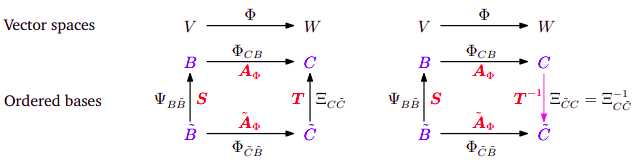
\includegraphics[
        width=\linewidth, 
        height=4cm,
        keepaspectratio,
    ]{images/maths-for-ml/basis-change.png}
    \caption*{
        For a homomorphism $\Phi  : V \to  W$ and ordered bases $B, \tilde{B}$ of $V$ and $C, \tilde{C}$ of $W$ (marked in \textcolor{blue}{blue}), we can express the mapping $\Phi _{\tilde{C} \tilde{B}}$ with respect to the bases $\tilde{B}, \tilde{C}$ equivalently as a composition of the homomorphisms $\Phi _{\tilde{C} \tilde{B}} = \Xi _{\tilde{C}C} \circ \Phi _{CB} \circ \Psi _{B\tilde{B}}$ with respect to the bases in the subscripts. 
        \\
        The corresponding transformation matrices are in \textcolor{red}{red}.
        \\
        We use $\Psi_{B\tilde{B}} = \text{id}_V$ and $\Xi _{C\tilde{C}} = \text{id}_W$ , i.e., the identity mappings that map vectors onto themselves, but with respect to a different basis.
        \hfill \cite{mfml/book/mml/Deisenroth-Faisal-Ong}
    }
\end{figure}


\begin{enumerate}
    \item
    \begin{theorem}[Basis Change]
        For a linear mapping $\Phi : V \to W$, ordered bases
        \hfill \cite{mfml/book/mml/Deisenroth-Faisal-Ong}
        \\
        .\hfill
        $
            B = (\bm{b}_1, \cdots , \bm{b}_n), \ 
            \tilde{B} = (\tilde{\bm{b}}_1, \cdots , \tilde{\bm{b}}_n)
        $
        \hfill \cite{mfml/book/mml/Deisenroth-Faisal-Ong}
        \\
        of $V$ and
        \hfill \cite{mfml/book/mml/Deisenroth-Faisal-Ong}
        \\
        .\hfill
        $
            C = (\bm{c}_1, \cdots , \bm{c}_n), \ 
            \tilde{C} = (\tilde{\bm{c}}_1, \cdots , \tilde{\bm{c}}_n)
        $
        \hfill \cite{mfml/book/mml/Deisenroth-Faisal-Ong}
        \\
        of $W$, and a transformation matrix $\bm{A}_\Phi$ of $\Phi$ with respect to $B$ and $C$, the corresponding transformation matrix $\tilde{\bm{A}} _\Phi$ with respect to the bases $\tilde{B}$ and $\tilde{C}$ is given as
        $
            \tilde{\bm{A}} \Phi = \bm{T}^{-1}\bm{A}_\Phi \bm{S}
        $.
        \hfill \cite{mfml/book/mml/Deisenroth-Faisal-Ong}
        \\
        Here, $\bm{S} \in \mathbb{R}^{n\times n}$ is the transformation matrix of $\text{id}_V$ that maps coordinates with respect to $\tilde{B}$ onto coordinates with respect to $B$, \ 
        and $\bm{T} \in \mathbb{R}^{m\times m}$ is the transformation matrix of $\text{id}_W$ that maps coordinates with respect to $\tilde{C}$ onto coordinates with respect to $C$.
        \hfill \cite{mfml/book/mml/Deisenroth-Faisal-Ong}
    \end{theorem}

    \begin{proof}
        we can write the vectors of the new basis $\tilde{B}$ of $V$ as a linear combination of the basis vectors of $B$, such that:
        \hfill \cite{mfml/book/mml/Deisenroth-Faisal-Ong}
        \\
        .\hfill
        $
            \tilde{\bm{b}}_j 
            = s_{1j} \bm{b}_1 + \cdots + s_{nj} \bm{b}_n 
            = \dsum^n _{i=1} s_{ij} \bm{b}_i 
            , j = 1, \cdots , n
        $
        \hfill \cite{mfml/book/mml/Deisenroth-Faisal-Ong}
        \\
        Similarly, we write the new basis vectors $\tilde{C}$ of $W$ as a linear combination of the basis vectors of $C$, which yields
        \hfill \cite{mfml/book/mml/Deisenroth-Faisal-Ong}
        \\
        .\hfill
        $
            \tilde{\bm{c}}_k 
            = t_{1k} \bm{c}_1 + \cdots + t_{mk} \bm{c}_m 
            = \dsum^m _{l=1} t_{lk} \bm{c}_l 
            , k = 1, \cdots , m
        $
        \hfill \cite{mfml/book/mml/Deisenroth-Faisal-Ong}
        \\
        We define $\bm{S} = ((s_{ij} )) \in \mathbb{R}^{n\times n}$ as the transformation matrix that maps coordinates with respect to $\tilde{B}$ onto coordinates with respect to $B$ and $\bm{T} = ((t_{lk})) \in R^{m\times m}$ as the transformation matrix that maps coordinates with respect to $\tilde{C}$ onto coordinates with respect to $C$. 
        In particular, the $j$-th column of $\bm{S}$ is the coordinate representation of $\tilde{\bm{b}}_j$ with respect to $B$ and the $k$-th column of $\bm{T}$ is the coordinate representation of $\tilde{\bm{c}}_k$ with respect to $C$. 
        Note that both $\bm{S}$ and $\bm{T}$ are regular.
        \hfill \cite{mfml/book/mml/Deisenroth-Faisal-Ong}
        \\
        We are going to look at $\Phi(\tilde{\bm{b}}_j )$ from two perspectives.
        \hfill \cite{mfml/book/mml/Deisenroth-Faisal-Ong}
        \begin{enumerate}
            \item Applying the mapping $\Phi$, we get that for all $j = 1, \cdots , n$
            \hfill \cite{mfml/book/mml/Deisenroth-Faisal-Ong}
            \\
            .\hfill
            $
                \Phi(\tilde{\bm{b}}_j )
                = \dsum^m_{k=1} \underset{\displaystyle \in W}{
                    \underbrace{\tilde{a}_{kj} \textcolor{blue}{\tilde{\bm{c}}_k}}
                }
                = \dsum^m_{k=1} \tilde{a}_{kj} \textcolor{blue}{
                    \dsum^m_{l=1} t_{lk} \bm{c}_l
                }
                = \dsum^m_{l=1} \dParenBrac{
                    \textcolor{PineGreen}{\dsum^m_{k=1} t_{lk} \tilde{a}_{kj}} 
                }  \bm{c}_l
            $
            \hfill \cite{mfml/book/mml/Deisenroth-Faisal-Ong}
            \\
            where we first expressed the new basis vectors $\tilde{\bm{c}}_k \in W$ as linear combinations of the basis vectors $\bm{c}_l \in W$ and then swapped the order of summation.
            \hfill \cite{mfml/book/mml/Deisenroth-Faisal-Ong}
    
    
            \item when we express the $\tilde{\bm{b}}_j \in V$ as linear combinations of $\bm{b}_j \in V$ , we arrive at ($j = 1,\cdots, n$) :
            \hfill \cite{mfml/book/mml/Deisenroth-Faisal-Ong}
            \\
            .\hfill
            $
                \Phi (\tilde{\bm{b}}_j ) 
                = \Phi  \dParenBrac{ \textcolor{blue}{\dsum ^n _{i=1} s_{ij} \bm{b}_i}}
                = \dsum ^n _{i=1} s_{ij} \textcolor{red}{\Phi (\bm{b}_i)} 
                = \dsum^n _{i=1} s_{ij} \textcolor{red}{\dsum ^m _{l=1} a_{li} \bm{c}_l}
                = \dsum ^m _{l=1} \dParenBrac{ \textcolor{PineGreen}{\dsum^n _{i=1} s_{ij} a_{li}} } \bm{c}_l
            $
            \hfill \cite{mfml/book/mml/Deisenroth-Faisal-Ong}
    
            \item $
                \begin{aligned}
                    \dsum^m_{k=1} t_{lk} \tilde{a}_{kj} = \dsum^n _{i=1} s_{ij} a_{li}
                    \hspace{1cm}
                    \Rightarrow 
                    \bm{T} \tilde{\bm{A}}_\Phi = \bm{A}_\Phi \bm{S} 
                    \in \mathbb{R}^{m\times n}
                    \hspace{1cm}
                    \Rightarrow 
                    \tilde{\bm{A}}_\Phi = \bm{T}^{-1} \bm{A}_\Phi \bm{S}
                \end{aligned}
            $
            \hfill \cite{mfml/book/mml/Deisenroth-Faisal-Ong}        
        \end{enumerate}
    \end{proof}

    
\end{enumerate}






\subsection{Orthonormal Basis (ONB) \& Orthogonal Basis (OGB)}


\begin{enumerate}
    \item
    \begin{definition}[Orthonormal Basis (ONB)]
        Consider an $n$-dimensional vector space $V$ and a basis $\dCurlyBrac{\bm{b}_1, \cdots , \bm{b}_n}$ of $V$ . 
        If
        \hfill \cite{mfml/book/mml/Deisenroth-Faisal-Ong}
        \\
        .\hfill
        $\dAngleBrac{\bm{b}_i, \bm{b}_j} = 0$ for $i \neq j$ and $\dAngleBrac{\bm{b}_i, \bm{b}_i} = 1$
        \hfill \cite{mfml/book/mml/Deisenroth-Faisal-Ong}
        \\
        for all $i, j = 1, \cdots , n$ then the basis is called an orthonormal basis (ONB).
        \hfill \cite{mfml/book/mml/Deisenroth-Faisal-Ong}
    \end{definition}

    \item If only $\dAngleBrac{\bm{b}_i, \bm{b}_j} = 0$ is satisfied, then the basis is called an \textbf{orthogonal basis}.
    \hfill \cite{mfml/book/mml/Deisenroth-Faisal-Ong}

    \item \textbf{Note}: $\dAngleBrac{\bm{b}_i, \bm{b}_i} = 1$ implies that every basis vector has length/norm $1$.
    \hfill \cite{mfml/book/mml/Deisenroth-Faisal-Ong}

\end{enumerate}

\subsubsection{Orthogonalization using Gaussian Elimination}

\begin{enumerate}
    \item constructive way to iteratively build an orthonormal basis
    \hfill \cite{mfml/book/mml/Deisenroth-Faisal-Ong}

    \item Assume we are given a set $\dCurlyBrac{\tilde{\bm{b}}_1, \cdots ,\tilde{\bm{b}}_n}$ of non-orthogonal and un-normalized basis vectors.
    \hfill \cite{mfml/book/mml/Deisenroth-Faisal-Ong}

    \item We concatenate them into a matrix $\tilde{\bm{B}} = [\tilde{\bm{b}}_1, \cdots ,\tilde{\bm{b}}_n]$ and apply Gaussian elimination to the augmented matrix $[\tilde{\bm{B}} \tilde{\bm{B}}^\top|\tilde{\bm{B}}]$ to obtain an orthonormal basis. 
    \hfill \cite{mfml/book/mml/Deisenroth-Faisal-Ong}
\end{enumerate}


\begin{lstlisting}[
    language=Python,
    caption=Orthogonalization using Gaussian Elimination - numPy
]
import numpy as np
from scipy.linalg import orth

def gram_schmidt_from_augmented_matrix(basis_vectors):
    """
    Implements Gram-Schmidt as described via augmented matrix [B B^T | B]

    Parameters:
        basis_vectors (list of np.ndarray): List of non-orthogonal 
            basis vectors (each of same length)

    Returns:
        np.ndarray: Matrix with orthonormal basis vectors as columns
    """
    # Step 1: Form B matrix from input list
    B = np.column_stack(basis_vectors)  # Shape: (d, n)

    # Step 2: Form the augmented matrix [B B^T | B]
    BB_T = B @ B.T                      # Shape: (d, d)
    augmented = np.hstack((BB_T, B))   # Shape: (d, d + n)

    # Step 3: Apply Gaussian elimination to the augmented matrix
    # Instead of manual row ops, we extract the column space of B using orth()
    # This gives us an orthonormal basis for the column space of B
    Q = orth(B)  # Shape: (d, r), where r = rank(B)

    return Q  # Orthonormal basis matrix


B_tilde = [
    np.array([1, 1, 0]),
    np.array([1, 0, 1]),
    np.array([0, 1, 1])
]

Q = gram_schmidt_from_augmented_matrix(B_tilde)

print("Orthonormal basis vectors:")
for i in range(Q.shape[1]):
    print(f"b_{i+1} =", Q[:, i])
\end{lstlisting}







\subsubsection{Gram-Schmidt Orthogonalization}


\begin{figure}[H]
    \centering
    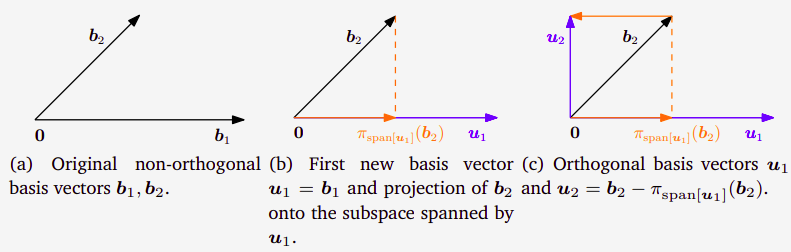
\includegraphics[
        width=\linewidth,
        height=4cm,
        keepaspectratio,
    ]{images/maths-for-ml/Gram-Schmidt-orthogonalization-eg-3.12.png}
    \caption*{
        Gram-Schmidt orthogonalization. 
        \hfill \cite{mfml/book/mml/Deisenroth-Faisal-Ong}
        \\
        (a) non-orthogonal basis $(\bm{b}_1, \bm{b}_2)$ of $\mathbb{R}^2$ 
        \hfill \cite{mfml/book/mml/Deisenroth-Faisal-Ong}
        \\
        (b) first constructed basis vector $\bm{u}_1$ and orthogonal projection of $\bm{b}_2$ onto $\text{span}[\bm{u}_1]$; 
        \hfill \cite{mfml/book/mml/Deisenroth-Faisal-Ong}
        \\
        (c) orthogonal basis $(\bm{u}_1, \bm{u}_2)$ of $\mathbb{R}^2$.
        \hfill \cite{mfml/book/mml/Deisenroth-Faisal-Ong}
    }
\end{figure}


\begin{enumerate}
    \item Method 1 
    \hfill \cite{mfml/book/mml/Deisenroth-Faisal-Ong}
    \\
    Projections are at the core of the Gram-Schmidt method that allows us to constructively transform any basis $(\bm{b}_1, \cdots , \bm{b}_n)$ of an $n$-dimensional vector space $V$ into an orthogonal/orthonormal basis $(\bm{u}_1, \cdots ,\bm{u}_n)$ of $V$ .
    This basis always exists and $\text{span}[\bm{b}_1, \cdots , \bm{b}_n] = \text{span}[\bm{u}_1, \cdots , \bm{u}_n]$.
    \hfill \cite{mfml/book/mml/Deisenroth-Faisal-Ong}
    \begin{enumerate}
        \item $\bm{u}_1 := \bm{b}_1$
        \hfill \cite{mfml/book/mml/Deisenroth-Faisal-Ong}

        \item $
            \bm{u}_k := \bm{b}_k - \pi_{\text{span}[\bm{u}_1,\cdots,\bm{u}_{k-1}]}(\bm{b}_k)
            \hspace{1cm}
            ,k = 2, \cdots , n
        $
        \hfill \cite{mfml/book/mml/Deisenroth-Faisal-Ong}
    \end{enumerate}
    the $k$-th basis vector $\bm{b}_k$ is projected onto the subspace spanned by the first $k - 1$ constructed orthogonal vectors $\bm{u}_1, \cdots ,\bm{u}_{k-1}$.
    If we normalize the $\bm{u}_k$, we obtain an ONB where $\dnorm{\bm{u}_k} = 1$ for $k = 1, \cdots , n$
    

    \item Method 2
    \hfill \cite{mfml/wiki/Gram-Schmidt_process}
    \begin{enumerate}
        \item ${
            \displaystyle 
            \operatorname {proj} _{\mathbf {u} }(\mathbf {b} )
            ={\frac {\langle \mathbf {v} ,\mathbf {b} \rangle }{\langle \mathbf {u} ,\mathbf {u} \rangle }}
            \,\mathbf {u} 
        }$
        \hfill \cite{mfml/wiki/Gram-Schmidt_process}

        \item ${
        \displaystyle 
        {\begin{aligned}
            \mathbf {u} _{1} &=\mathbf {b} _{1}, &\!\mathbf {e} _{1}&={\frac {\mathbf {u} _{1}}{\|\mathbf {u} _{1}\|}}
            \\\mathbf {u} _{2}&=\mathbf {b} _{2}-\operatorname {proj} _{\mathbf {u} _{1}}(\mathbf {b} _{2}),&\!\mathbf {e} _{2}&={\frac {\mathbf {u} _{2}}{\|\mathbf {u} _{2}\|}}
            \\\mathbf {u} _{3}&=\mathbf {b} _{3}-\operatorname {proj} _{\mathbf {u} _{1}}(\mathbf {b} _{3})-\operatorname {proj} _{\mathbf {u} _{2}}(\mathbf {b} _{3}),&\!\mathbf {e} _{3}&={\frac {\mathbf {u} _{3}}{\|\mathbf {u} _{3}\|}}
            \\\mathbf {u} _{4}&=\mathbf {b} _{4}-\operatorname {proj} _{\mathbf {u} _{1}}(\mathbf {b} _{4})-\operatorname {proj} _{\mathbf {u} _{2}}(\mathbf {b} _{4})-\operatorname {proj} _{\mathbf {u} _{3}}(\mathbf {b} _{4}),&\!\mathbf {e} _{4}&={\mathbf {u} _{4} \over \|\mathbf {u} _{4}\|}
            \\&{}\ \ \vdots &&{}\ \ \vdots 
            \\\mathbf {u} _{k}&=\mathbf {b} _{k}-\sum _{j=1}^{k-1}\operatorname {proj} _{\mathbf {u} _{j}}(\mathbf {b} _{k}),&\!\mathbf {e} _{k}&={\frac {\mathbf {u} _{k}}{\|\mathbf {u} _{k}\|}}
        \end{aligned}}
        }$
        \hfill \cite{mfml/wiki/Gram-Schmidt_process}
    \end{enumerate}
    The sequence ${\displaystyle \mathbf {u} _{1},\ldots ,\mathbf {u} _{k}}$ is the required system of orthogonal vectors, and the normalized vectors ${\displaystyle \mathbf {e} _{1},\ldots ,\mathbf {e} _{k}}$ form an orthonormal set. 
    \hfill \cite{mfml/wiki/Gram-Schmidt_process}
\end{enumerate}


\begin{lstlisting}[
    language=Python,
    caption=Gram-Schmidt Orthogonalization \& Orthonormalization - numPy
]
import numpy as np

def gram_schmidt(vectors, inner_product=None):
    """
    Perform Gram-Schmidt orthogonalization on a list of vectors.

    Parameters:
        vectors (list of np.ndarray): List of n vectors in R^d 
            (each a 1D array).
        inner_product (function): Function to 
            compute inner product, default is np.dot.

    Returns:
        orthogonal_basis (list of np.ndarray): Orthogonal 
            (not normalized) basis vectors.
    """

    if inner_product is None:
        inner_product = lambda u, v: np.dot(u, v)

    orthogonal_basis = []

    for i, v in enumerate(vectors):
        v_proj = np.zeros_like(v)
        for u in orthogonal_basis:
            proj_coeff = inner_product(v, u) / inner_product(u, u)
            v_proj += proj_coeff * u
        u_i = v - v_proj
        orthogonal_basis.append(u_i)

    return orthogonal_basis


def normalize_vectors(vectors, norm=None):
    """
    Normalize a list of vectors using the given norm.

    Parameters:
        vectors (list of np.ndarray): List of vectors to normalize.
        norm (function): Norm function, default is np.linalg.norm.

    Returns:
        list of np.ndarray: Normalized vectors.
    """
    if norm is None:
        norm = lambda v: np.linalg.norm(v)
    return [v / norm(v) for v in vectors]


# Define basis vectors in R^2
b1 = np.array([1.0, 1.0])
b2 = np.array([1.0, 0.0])

basis = [b1, b2]

# Use standard inner product and norm
orthogonal_basis = gram_schmidt(basis)
orthonormal_basis = normalize_vectors(orthogonal_basis)

print("Orthogonal basis:")
for v in orthogonal_basis:
    print(v)

print("\nOrthonormal basis:")
for v in orthonormal_basis:
    print(v)

###### custom inner product/ norm

# Weighted inner product with weight matrix W
W = np.array([[2, 0], [0, 3]])
def weighted_inner(u, v):
    return np.dot(u.T, W @ v)

# Weighted norm (induced by W)
def weighted_norm(v):
    return np.sqrt(weighted_inner(v, v))

orthogonal_basis = gram_schmidt(basis, inner_product=weighted_inner)
orthonormal_basis = normalize_vectors(orthogonal_basis, norm=weighted_norm)

print("Orthogonal basis:")
for v in orthogonal_basis:
    print(v)

print("\nOrthonormal basis:")
for v in orthonormal_basis:
    print(v)
\end{lstlisting}

output:
\begin{lstlisting}[
    % language=Python,
    % caption=Gram-Schmidt Orthogonalization \& Orthonormalization - numPy
]
Orthogonal basis:
[1. 1.]
[ 0.5 -0.5]

Orthonormal basis:
[0.70710678 0.70710678]
[ 0.70710678 -0.70710678]

Orthogonal basis:
[1. 1.]
[ 0.6 -0.4]

Orthonormal basis:
[0.4472136 0.4472136]
[ 0.54772256 -0.36514837]
\end{lstlisting}























\section{Linear Mappings ($\Phi$)}


\begin{figure}[H]
    \centering
    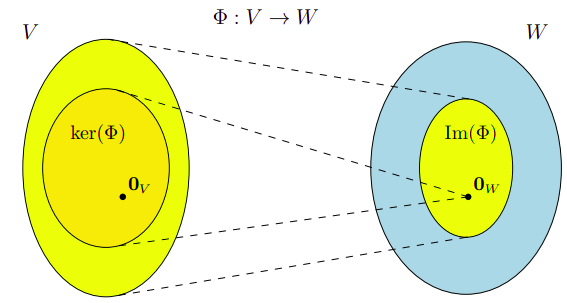
\includegraphics[
        width=\linewidth,
        height=4cm,
        keepaspectratio,
    ]{images/maths-for-ml/image-kernel-linear-mapping.png}
\end{figure}

\begin{enumerate}
    \item
    \begin{definition}[Linear Mapping]
        For vector spaces $V, W$, a mapping $\Phi : V \to W$ is called a linear mapping (or vector space homomorphism/ linear transformation) if
        \hfill \cite{mfml/book/mml/Deisenroth-Faisal-Ong}
        \\
        .\hfill
        $
            \forall \bm{x}, \bm{y} \in V \forall \lambda , \psi  \in \mathbb{R} : 
            \Phi(\lambda \bm{x} + \psi \bm{y}) = \lambda \Phi(\bm{x}) + \psi \Phi(\bm{y})
        $
        \hfill \cite{mfml/book/mml/Deisenroth-Faisal-Ong}
    \end{definition}

    \item we can represent linear mappings as matrices
    \hfill \cite{mfml/book/mml/Deisenroth-Faisal-Ong}

    \item For linear mappings $\Phi : V \to W$ and $\Psi : W \to X$, the mapping $\Psi \circ \Phi : V \to X$ is also linear.
    \hfill \cite{mfml/book/mml/Deisenroth-Faisal-Ong}

    \item If $\Phi : V \to W, \Psi : V \to W$ are linear, then $\Phi + \Psi$ and $\lambda\Phi, \lambda \in \mathbb{R}$, are linear, too.
    \hfill \cite{mfml/book/mml/Deisenroth-Faisal-Ong}
\end{enumerate}



\subsection{Matrix Representation of Linear Mappings}

\begin{enumerate}
    \item Any $n$-dimensional vector space is isomorphic to $\mathbb{R}^n$.
    \hfill \cite{mfml/book/mml/Deisenroth-Faisal-Ong}

    \item We consider a basis $\dCurlyBrac{\bm{b}_1, \cdots , \bm{b}_n}$ of an $n$-dimensional vector space $V$ .
    \hfill \cite{mfml/book/mml/Deisenroth-Faisal-Ong}
\end{enumerate}




\subsection{Image/Range \& Kernel/Null space}

\begin{enumerate}
    \item
    \begin{definition}[Image/ Range]
        For $\Phi  : V \to W$, we define the image/range
        \hfill \cite{mfml/book/mml/Deisenroth-Faisal-Ong}
        \\
        .\hfill
        $
            \text{Im}(\Phi ) 
            := \Phi (V ) 
            = \dCurlyBrac{\bm{w} \in W|\exists \bm{v} \in V : \Phi (\bm{v}) = \bm{w}}
        $
        \hfill \cite{mfml/book/mml/Deisenroth-Faisal-Ong}
    \end{definition}

    \item
    \begin{definition}[Kernel/ Null Space]
        For $\Phi  : V \to W$, we define the kernel/null space
        \hfill \cite{mfml/book/mml/Deisenroth-Faisal-Ong}
        \\
        .\hfill
        $
            \ker(\Phi ) 
            := \Phi ^{-1} (\bm{0}_W ) 
            = \dCurlyBrac{\bm{v} \in V : \Phi (\bm{v}) = \bm{0}_W }
        $
        \hfill \cite{mfml/book/mml/Deisenroth-Faisal-Ong}
    \end{definition}


    \item We also call $V$ and $W$ also the \textbf{domain} and \textbf{codomain} of $\Phi$, respectively.
    \hfill \cite{mfml/book/mml/Deisenroth-Faisal-Ong}

    \item The image is the set of vectors $\bm{w} \in W$ that can be “reached” by $\Phi$ from any vector in $V$ .
    \hfill \cite{mfml/book/mml/Deisenroth-Faisal-Ong}

    \item Intuitively, the kernel is the set of vectors $\bm{v} \in V$ that $\Phi$ maps onto the neutral element $\bm{0}_W \in W$.
    \hfill \cite{mfml/book/mml/Deisenroth-Faisal-Ong}

    \item It always holds that $\Phi(\bm{0}_V ) = \bm{0}_W$ and, therefore, $\bm{0}_V \in \ker(\Phi)$. 
    In particular, the null space is never empty.
    \hfill \cite{mfml/book/mml/Deisenroth-Faisal-Ong}

    \item $Im(\Phi) \subseteq W$ is a subspace of $W$, and $\ker(\Phi) \subseteq V$ is a subspace of $V$ .
    \hfill \cite{mfml/book/mml/Deisenroth-Faisal-Ong}

    \item $\Phi$ is injective (one-to-one) if and only if $\ker(\Phi) = \dCurlyBrac{\bm{0}}$.
    \hfill \cite{mfml/book/mml/Deisenroth-Faisal-Ong}

    \item
    \begin{theorem}[Rank-Nullity Theorem]
        For vector spaces $V, W$ and a linear mapping $\Phi : V \to W$ it holds that $\dim(\ker(\Phi)) + \dim(\text{Im}(\Phi)) = \dim(V )$.
        \hfill \cite{mfml/book/mml/Deisenroth-Faisal-Ong}
    \end{theorem}
    \begin{enumerate}
        \item The rank-nullity theorem is also referred to as the \textbf{fundamental theorem of linear mappings}
        \hfill \cite{mfml/book/mml/Deisenroth-Faisal-Ong}

        \item If $\dim(\text{Im}(\Phi )) < \dim(V )$, then $\ker(\Phi)$ is non-trivial, i.e., the kernel contains more than $\bm{0}_V$ and $\dim(\ker(\Phi)) \geq 1$.
        \hfill \cite{mfml/book/mml/Deisenroth-Faisal-Ong}

        \item If $\bm{A}_\Phi $ is the transformation matrix of $\Phi$  with respect to an ordered basis and $\dim(\text{Im}(\Phi )) < \dim(V )$, then the system of linear equations $\bm{A}_\Phi \bm{x} = \bm{0}$ has infinitely many solutions.
        \hfill \cite{mfml/book/mml/Deisenroth-Faisal-Ong}

        \item If $\dim(V ) = \dim(W)$, then the following three-way equivalence holds:
        \begin{enumerate}
            \item $\Phi$ is injective
            \item $\Phi$ is surjective
            \item $\Phi$ is bijective
        \end{enumerate}
        since $\text{Im}(\Phi) \subseteq W$.
    \end{enumerate}
\end{enumerate}













\section{Affine Mapping}

\begin{enumerate}
    \item
    \begin{definition}[Affine Mapping]
        For two vector spaces $V, W$, a linear mapping $\Phi : V \to W$, and $\bm{a} \in W$, the mapping:
        \hfill \cite{mfml/book/mml/Deisenroth-Faisal-Ong}
        \\
        .\hfill
        $ \phi : V \to W $ such that $ \bm{x} \mapsto \bm{a} + \Phi(\bm{x}) $
        \hfill \cite{mfml/book/mml/Deisenroth-Faisal-Ong}
        \\
        is an affine mapping from $V$ to $W$. 
        The vector a is called the \textbf{translation vector} of $\phi$.
        \hfill \cite{mfml/book/mml/Deisenroth-Faisal-Ong}
    \end{definition}

    \item Every affine mapping $\phi  : V \to W$ is also the composition of a linear mapping $\phi  : V \to W$ and a translation $\tau : W \to W$ in $W$, such that $\phi  = \tau \circ \phi $. 
    The mappings $\phi $ and $\tau$ are uniquely determined.
    \hfill \cite{mfml/book/mml/Deisenroth-Faisal-Ong}

    \item The composition $\phi ^\prime \circ \phi $ of affine mappings $\phi  : V \to W, \phi ^\prime: W \to X$ is affine.
    \hfill \cite{mfml/book/mml/Deisenroth-Faisal-Ong}

    \item Affine mappings keep the geometric structure invariant. 
    They also preserve the dimension and parallelism.
    \hfill \cite{mfml/book/mml/Deisenroth-Faisal-Ong}
\end{enumerate}



























\section{Injective, Surjective, Bijective Mappings}

Consider a mapping $\Phi : \mathcal{V} \to \mathcal{W}$, where $\mathcal{V}, \mathcal{W}$ can be arbitrary sets. 
Then $\Phi$ is called:
\hfill \cite{mfml/book/mml/Deisenroth-Faisal-Ong}

\begin{enumerate}
    \item 
    \begin{definition}[Injective] 
        if $\forall \bm{x}, \bm{y} \in \mathcal{V} : \Phi(\bm{x}) = \Phi(\bm{y}) \Rightarrow \bm{x} = \bm{y}$
        \hfill \cite{mfml/book/mml/Deisenroth-Faisal-Ong}
    \end{definition}

    \item 
    \begin{definition}[Surjective]
        if $\Phi(\mathcal{V}) = \mathcal{W}$
        \hfill \cite{mfml/book/mml/Deisenroth-Faisal-Ong}
    \end{definition}
    \begin{enumerate}
        \item If $\Phi$ is surjective, then every element in $\mathcal{W}$ can be “reached” from $\mathcal{V}$ using $\Phi$.
        \hfill \cite{mfml/book/mml/Deisenroth-Faisal-Ong}
    \end{enumerate}
    
    \item 
    \begin{definition}[Bijective]
        if it is injective and surjective
        \hfill \cite{mfml/book/mml/Deisenroth-Faisal-Ong}
    \end{definition}
    \begin{enumerate}
        \item A bijective $\Phi$ can be “undone”, i.e., there exists a mapping $\Psi : W \to V$ so that $\Psi \circ \Phi(\bm{x}) = \bm{x}$.
        \hfill \cite{mfml/book/mml/Deisenroth-Faisal-Ong}

        \item This mapping $\Psi$ is then called the inverse of $\Phi$ and normally denoted by $\Phi^{-1}$.
        \hfill \cite{mfml/book/mml/Deisenroth-Faisal-Ong}
    \end{enumerate}    

\end{enumerate}


















\section{Special cases of Linear mappings}

Consider a mapping $\Phi : V \to W$, where $V, W$ can be arbitrary vector spaces. 
Then:
\hfill \cite{mfml/book/mml/Deisenroth-Faisal-Ong}

\begin{enumerate}
    \item 
    \begin{definition}[Isomorphism]
        $\Phi : V \to W$ linear and bijective
        \hfill \cite{mfml/book/mml/Deisenroth-Faisal-Ong}
    \end{definition}
    \begin{enumerate}
        \item
        \begin{theorem}[isomorphic vector spaces]
            Finite-dimensional vector spaces $V$ and $W$ are isomorphic if and only if $\dim(V ) = \dim(W)$.
            \hfill \cite{mfml/book/mml/Deisenroth-Faisal-Ong}
        \end{theorem}

        \item there exists a linear, bijective mapping between two vector spaces of the same dimension.
        Intuitively, this means that vector spaces of the same dimension are kind of the same thing, as they can be transformed into each other without incurring any loss.
        \hfill \cite{mfml/book/mml/Deisenroth-Faisal-Ong}

        \item It gives the justification to treat $\mathbb{R}^{m\times n}$ (the vector space of $m \times n$-matrices) and $\mathbb{R}^{mn}$ (the vector space of vectors of length $mn$) the same, as their dimensions are $mn$, and there exists a linear, bijective mapping that transforms one into the other.
        \hfill \cite{mfml/book/mml/Deisenroth-Faisal-Ong}

        \item If $\Phi : V \to W$ is an isomorphism, then $\Phi ^{-1} : W \to V$ is an isomorphism, too.
        \hfill \cite{mfml/book/mml/Deisenroth-Faisal-Ong}
    \end{enumerate}

    \item 
    \begin{definition}[Endomorphism]
        $\Phi : V \to V$ linear
        \hfill \cite{mfml/book/mml/Deisenroth-Faisal-Ong}
    \end{definition}

    \item 
    \begin{definition}[Automorphism]
        $\Phi : V \to V$ linear and bijective
        \hfill \cite{mfml/book/mml/Deisenroth-Faisal-Ong}
    \end{definition}

    \item 
    \begin{definition}[identity mapping/ identity automorphism]
        $id_V : V \to V , \bm{x} \mapsto \bm{x}$
        \hfill \cite{mfml/book/mml/Deisenroth-Faisal-Ong}
    \end{definition}
\end{enumerate}



















\section{Transformation Matrix ( $A_\Phi$ )}

\begin{enumerate}
    \item 
    \begin{definition}[Transformation Matrix]
        Consider vector spaces $V$, $W$ with corresponding (ordered) bases $B = (\bm{b}_1, \cdots , \bm{b}_n)$ and $C = (\bm{c}_1, \cdots , \bm{c}_m)$. 
        Moreover, we consider a linear mapping $\Phi : V \to W$. 
        For $j \in \dCurlyBrac{1, \cdots , n}$,
        \hfill \cite{mfml/book/mml/Deisenroth-Faisal-Ong}
        \\
        .\hfill
        $
            \Phi(\bm{b}_j ) = \alpha _{1j} \bm{c}_1 + \cdots + \alpha _{mj} \bm{c}_m 
            = \dsum^m_{i=1} \alpha _{ij} \bm{c}_i
        $
        \hfill \cite{mfml/book/mml/Deisenroth-Faisal-Ong}
        \\
        is the unique representation of $\Phi(\bm{b}_j )$ with respect to $C$. 
        Then, we call the $m \times n$-matrix $\bm{A}_\Phi$, whose elements are given by $\bm{A}_\Phi(i, j) = \alpha_{ij}$ the transformation matrix of $\Phi$ (with respect to the ordered bases $B$ of $V$ and $C$ of $W$  ).
        \hfill \cite{mfml/book/mml/Deisenroth-Faisal-Ong}
    \end{definition}

    \item The transformation matrix can be used to map coordinates with respect to an ordered basis in $V$ to coordinates with respect to an ordered basis in $W$.
    \hfill \cite{mfml/book/mml/Deisenroth-Faisal-Ong}

    \item Consider vector spaces $V, W, X$. 
    We already know that for linear mappings $\Phi  : V \to  W$ and $\Psi : W \to  X$ the mapping $\Psi \circ \Phi  : V \to  X$ is also linear. 
    With transformation matrices $\bm{A}_\Phi$  and $\bm{A}_\Psi$ of the corresponding mappings, the overall transformation matrix is $\bm{A}_{\Psi\circ\Phi}  = \bm{A}_\Psi \bm{A}_\Phi$ .
    \hfill \cite{mfml/book/mml/Deisenroth-Faisal-Ong}

    \item 
    $\bm{A}_\Phi$  is the transformation matrix of a linear mapping $\Phi _{CB} : V \to  W$ with respect to the bases $B, C$.
    \hfill \cite{mfml/book/mml/Deisenroth-Faisal-Ong}
    \\[0.2cm]
    $\tilde{\bm{A}}_\Phi$  is the transformation matrix of the linear mapping $\Phi_ {\tilde{C}\tilde{B}} : V \to  W$ with respect to the bases $\tilde{B}, \tilde{C}$.
    \hfill \cite{mfml/book/mml/Deisenroth-Faisal-Ong}
    \\[0.2cm]
    $\bm{S}$ is the transformation matrix of a linear mapping $\Psi _{B\tilde{B}} : V \to  V$ (automorphism) that represents $\tilde{B}$ in terms of $B$. Normally, $\Psi  = \text{id}_V$ is the identity mapping in $V$ .
    \hfill \cite{mfml/book/mml/Deisenroth-Faisal-Ong}
    \\[0.2cm]
    $\bm{T}$ is the transformation matrix of a linear mapping $\Xi _{C\tilde{C}} : W \to  W$ (automorphism) that represents $\tilde{C}$ in terms of $C$. Normally, $\Xi  = \text{id}_W$ is the identity mapping in $W$.
    \hfill \cite{mfml/book/mml/Deisenroth-Faisal-Ong}
    \\[0.2cm]
    If we (informally) write down the transformations just in terms of bases, then $\bm{A}_\Phi  : B \to  C$, $\tilde{\bm{A}}_\Phi  : \tilde{B} \to  \tilde{C}$, $\bm{S} : \tilde{B} \to  B$, $\bm{T} : \tilde{C} \to  C$ and $\bm{T}^{-1} : C \to  \bm{C}$, and
    \hfill \cite{mfml/book/mml/Deisenroth-Faisal-Ong}
    \\[0.2cm]
    .\hfill
    $
        \tilde{B} \to  \tilde{C} = \textcolor{blue}{\tilde{B} \to  B} \textcolor{red}{\to  C} \to  \tilde{C} 
        \Rightarrow
        \tilde{\bm{A}}_\Phi  = \bm{T}^{-1} \textcolor{red}{\bm{A}_\Phi} \textcolor{blue}{\bm{S}}
    $
    \hfill \cite{mfml/book/mml/Deisenroth-Faisal-Ong}
    \\[0.2cm]
    Note that the execution order is from \textbf{right to left} because vectors are multiplied at the right-hand side so that 
    \hfill \cite{mfml/book/mml/Deisenroth-Faisal-Ong}
    \\[0.2cm]
    .\hfill
    $\bm{x} \mapsto  \bm{Sx} \mapsto  \bm{A}_\Phi (\bm{Sx}) \mapsto \bm{T}^{-1}(\bm{A}_\Phi (\bm{Sx})) = \tilde{\bm{A}}_\Phi \bm{x}$.
    \hfill \cite{mfml/book/mml/Deisenroth-Faisal-Ong}

    \item  Orthogonal matrices define transformations that are rotations (with the possibility of flips).
    \hfill \cite{mfml/book/mml/Deisenroth-Faisal-Ong}
\end{enumerate}






\section{Coordinates}

\begin{enumerate}
    \item Consider a vector space $V$ and an ordered basis $B = (\bm{b}_1, \cdots , \bm{b}_n)$ of $V$ . 
    For any $\bm{x} \in V$ we obtain a unique representation (linear combination):
    \hfill \cite{mfml/book/mml/Deisenroth-Faisal-Ong}
    \\
    .\hfill
    $
        \bm{x} = \alpha_1 \bm{b}_1 + \cdots + \alpha_n \bm{b}_n
    $
    \hfill \cite{mfml/book/mml/Deisenroth-Faisal-Ong}
    \\
    of $\bm{x}$ with respect to $B$. 
    Then $\alpha_1, \cdots , \alpha_n$ are the coordinates of $\bm{x}$ with respect to $B$, and the vector:
    \hfill \cite{mfml/book/mml/Deisenroth-Faisal-Ong}
    \\
    .\hfill
    $
        \bm{\alpha} = \begin{bmatrix}
            \alpha_1 \\
            \vdots \\
            \alpha_n
        \end{bmatrix}
        \in \mathbb{R}^n
    $
    \hfill \cite{mfml/book/mml/Deisenroth-Faisal-Ong}
    \\
    is the \textbf{coordinate vector/ coordinate} representation of $\bm{x}$ with respect to the ordered basis $B$.
    \hfill \cite{mfml/book/mml/Deisenroth-Faisal-Ong}

    \item A basis effectively defines a coordinate system.
    \hfill \cite{mfml/book/mml/Deisenroth-Faisal-Ong}

    \item For an $n$-dimensional vector space $V$ and an ordered basis $B$ of $V$ , the mapping $\Phi : \mathbb{R}^n \to V , \Phi(\bm{e}_i) = \bm{b}_i , i = 1, \cdots , n$, is linear, where $(\bm{e}_1, \cdots , \bm{e}_n)$ is the standard basis of $\mathbb{R}^n$.
    \hfill \cite{mfml/book/mml/Deisenroth-Faisal-Ong}

    \item The coordinates of $\Phi(\bm{b}_j )$ with respect to the ordered basis $C$ of $W$ are the $j$-th column of $\bm{A}_\Phi$.
    \hfill \cite{mfml/book/mml/Deisenroth-Faisal-Ong}
    \hfill \cite{mfml/book/mml/Deisenroth-Faisal-Ong}
    \begin{enumerate}
        \item Consider (finite-dimensional) vector spaces $V$, $W$ with ordered bases $B$, $C$ and a linear mapping $\Phi : V \to W$ with transformation matrix $\bm{A}_\Phi$.
        \hfill \cite{mfml/book/mml/Deisenroth-Faisal-Ong}

        \item If $\hat{\bm{x}}$ is the coordinate vector of $\bm{x} \in V$ with respect to $B$ and $\hat{\bm{y}}$ the coordinate vector of $\bm{y} = \Phi(\bm{x}) \in W$ with respect to $C$, then $\hat{\bm{y}} = \bm{A}_\Phi \hat{\bm{x}}$.
        \hfill \cite{mfml/book/mml/Deisenroth-Faisal-Ong}
    \end{enumerate}    
\end{enumerate}












\section{Projections ( $\pi$ )}

\begin{enumerate}
    \item Projections are an important class of linear transformations (besides rotations and reflections) and play an important role in graphics, coding theory, statistics and machine learning.
    \hfill \cite{mfml/book/mml/Deisenroth-Faisal-Ong}

    \item High-dimensional data is often hard to analyze or visualize. 
    However, high-dimensional data quite often possesses the property that only a few dimensions contain most information, and most other dimensions are not essential to describe key properties of the data. 
    \hfill \cite{mfml/book/mml/Deisenroth-Faisal-Ong}

    \item When we compress or visualize high-dimensional data, we will lose information. To minimize this compression loss, we ideally find the most informative dimensions in the data.
    \hfill \cite{mfml/book/mml/Deisenroth-Faisal-Ong}

    \item we can project the original high-dimensional data onto a lower-dimensional \textbf{feature space} and work in this lower-dimensional space to learn more about the dataset and extract relevant patterns.
    \hfill \cite{mfml/book/mml/Deisenroth-Faisal-Ong}

    \item its a technique for dimensionality reduction.
    \hfill \cite{mfml/book/mml/Deisenroth-Faisal-Ong}

    \item For a given lower-dimensional subspace, orthogonal projections of high-dimensional data retain as much information as possible and minimize the difference/ error between the original data and the corresponding projection.
    \hfill \cite{mfml/book/mml/Deisenroth-Faisal-Ong}

    \item 
    \begin{definition}[projection]
        Let $V$ be a vector space and $U \subseteq V$ a subspace of $V$ . 
        A linear mapping $\pi : V \to U$ is called a projection if $\pi^2 = \pi \circ \pi = \pi$.
        \hfill \cite{mfml/book/mml/Deisenroth-Faisal-Ong}
    \end{definition}

    \item Any projection $\pi_U (\bm{x})$ onto $U$ is necessarily an element of $U$.
    Therefore, they can be represented as linear combinations of the basis vectors $\bm{b}_1, \cdots , \bm{b}_m$ of $U$, such that $\pi_U (\bm{x}) = \dsum ^m _{i=1} \lambda_i \bm{b}_i$.
    \hfill \cite{mfml/book/mml/Deisenroth-Faisal-Ong}

    \item 
    \begin{definition}[Projection error/ reconstruction error]
        The corresponding projection error is the norm of the difference vector between the original vector and its projection onto $U$: 
        $
            \dnorm{\bm{x} - \pi_U(\bm{x})}
        $
        \hfill \cite{mfml/book/mml/Deisenroth-Faisal-Ong}
    \end{definition}

    \item The projections $\pi_U (\bm{x})$ are still vectors in $\mathbb{R}^n$ although they lie in an $m$-dimensional subspace $U \subseteq \mathbb{R}^n$ . 
    However, to represent a projected vector we only need the $m$ coordinates $\lambda_1, \cdots , \lambda_m$ with respect to the basis vectors $\bm{b}_1, \cdots , \bm{b}_m$ of $U$.
    \hfill \cite{mfml/book/mml/Deisenroth-Faisal-Ong}

    \item If the basis $\bm{B}$ is an ONB, the projection equation 
    $
        \pi_U (\bm{x}) 
        = \bm{B} (\bm{B}^\top \bm{B})^{-1} \bm{B}^\top \bm{x}
    $
    simplifies greatly to $ \pi_U (\bm{x}) = \bm{B}\bm{B}^\top \bm{x}$ since $\bm{B}^\top \bm{B} = \bm{I}$ with coordinates $\bm{\lambda} = \bm{B}^\top \bm{x} $
\end{enumerate}



\subsection{Projection Matrix ( $P_\pi$ )}

\begin{enumerate}
    \item Since linear mappings can be expressed by transformation matrices, the definition of projection applies equally to a special kind  of transformation matrices, the projection matrices $\bm{P}_\pi$, which exhibit the property that $\bm{P}^2_\pi = \bm{P}_\pi$.
    \hfill \cite{mfml/book/mml/Deisenroth-Faisal-Ong}

    \item Projection matrices are always \textbf{symmetric}.
    \hfill \cite{mfml/book/mml/Deisenroth-Faisal-Ong}

    \item The projection matrix $\bm{P}_ \pi$ projects any vector $\bm{x} \in \mathbb{R}^n$ onto the line through the origin with direction $\bm{b}$ (equivalently, the subspace $U$ spanned by $\bm{b}$).
    \hfill \cite{mfml/book/mml/Deisenroth-Faisal-Ong}

    \item $\pi_U (\bm{x})$ is an eigenvector of $\bm{P}_\pi$, and the corresponding eigenvalue is $1$.
    \hfill \cite{mfml/book/mml/Deisenroth-Faisal-Ong}
\end{enumerate}



\subsection{Projection onto One-Dimensional Subspaces (Lines)}

\begin{table}[H]
\begin{minipage}{0.45\linewidth}
    \begin{figure}[H]
        \centering
        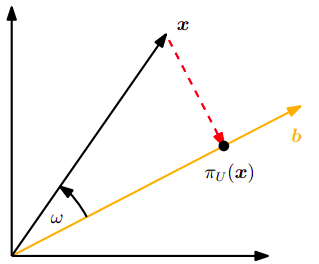
\includegraphics[
            width=\linewidth,
            height=4cm, 
            keepaspectratio,
        ]{images/maths-for-ml/Projection-1d-a.png}
        \caption*{
            Projection of $\bm{x} \in \mathbb{R}^2$ onto a subspace $U$ with basis vector $\bm{b}$.
            \cite{mfml/book/mml/Deisenroth-Faisal-Ong}
        }
    \end{figure}
\end{minipage}
\hfill
\begin{minipage}{0.45\linewidth}
    \begin{figure}[H]
        \centering
        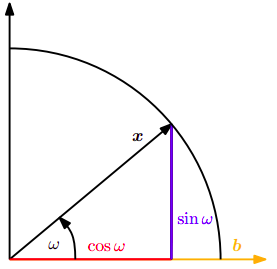
\includegraphics[
            width=\linewidth,
            height=4cm, 
            keepaspectratio,
        ]{images/maths-for-ml/Projection-1d-b.png}
        \caption*{
            Projection of a two-dimensional vector $\bm{x}$ with $\dnorm{\bm{x}} = 1$ onto a one-dimensional subspace spanned by $\bm{b}$.
            \cite{mfml/book/mml/Deisenroth-Faisal-Ong}
        }
    \end{figure}
\end{minipage}
\end{table}


\begin{enumerate}
    \item Assume we are given a line (one-dimensional subspace) through the origin with basis vector $\bm{b} \in \mathbb{R}^n$.
    The line is a one-dimensional subspace $U \subseteq \mathbb{R}^n$ spanned by $\bm{b}$. 
    \hfill \cite{mfml/book/mml/Deisenroth-Faisal-Ong}

    \item When we project $\bm{x} \in \mathbb{R}^n$ onto $U$, we seek the vector $\pi_U (\bm{x}) \in U$ that is closest to $\bm{x}$.
    \hfill \cite{mfml/book/mml/Deisenroth-Faisal-Ong}

    \item properties of the projection $\pi_U (\bm{x})$:
    \begin{enumerate}
        \item The projection $\pi _U (\bm{x})$ is closest to $\bm{x}$, where “closest” implies that the distance $\dnorm{\bm{x} - \pi _U (\bm{x})}$ is minimal. 
        It follows that the segment $\pi _U (\bm{x}) - x$ from $\pi _U (\bm{x})$ to $\bm{x}$ is orthogonal to $U$, and therefore the basis vector $\bm{b}$ of $U$. 
        The orthogonality condition yields $\dAngleBrac{\pi _U (\bm{x})  -  \bm{x}, \bm{b}} = 0$ since angles between vectors are defined via the inner product.
        \hfill \cite{mfml/book/mml/Deisenroth-Faisal-Ong}

        \item The projection $\pi_U (\bm{x})$ of $\bm{x}$ onto $U$ must be an element of $U$ and, therefore, a multiple of the basis vector $\bm{b}$ that spans $U$. 
        Hence, $\pi_U (\bm{x}) = \lambda\bm{b}$, for some $\lambda \in \mathbb{R}$.
        \hfill \cite{mfml/book/mml/Deisenroth-Faisal-Ong}
    \end{enumerate}

    \item Steps to determine $\lambda$, the projection $\pi _U (\bm{x}) \in  U$, and the projection matrix $\bm{P}_ \pi $ that maps any $\bm{x} \in  \mathbb{R}^n$ onto $U$:
    \hfill \cite{mfml/book/mml/Deisenroth-Faisal-Ong}
    \begin{enumerate}
        \item Finding the coordinate $\lambda $:
        \hfill \cite{mfml/book/mml/Deisenroth-Faisal-Ong}
        \\
        $
            \begin{aligned}
                & \dAngleBrac{\bm{x} - \pi_ U (x), \bm{b}} = 0 
                \\
                \Longleftrightarrow &
                    \dAngleBrac{\bm{x} - \lambda \bm{b}, \bm{b}} = 0
                    \Longleftrightarrow 
                    \dAngleBrac{\bm{x}, \bm{b}} - \lambda  \dAngleBrac{\bm{b}, \bm{b}} = 0 
                \\
                \Longleftrightarrow &
                    \lambda  
                    = \dfrac{\dAngleBrac{\bm{x}, \bm{b}}}{\dAngleBrac{\bm{b}, \bm{b}}} 
                    = \dfrac{\dAngleBrac{\bm{b}, \bm{x}}}{\dnorm{\bm{b}}^2}
                    \Longleftrightarrow 
                    \lambda 
                    =\dfrac{\bm{b}^\top \bm{x}}{\bm{b}^\top \bm{b}}
                    =\dfrac{\bm{b}^\top \bm{x}}{\dnorm{\bm{b}}^2}
            \end{aligned}
        $
        \hfill \cite{mfml/book/mml/Deisenroth-Faisal-Ong}
        \\
        If $\dnorm{\bm{b}} = 1$, then the coordinate $\lambda$ of the projection is given by $\bm{b}^\top \bm{x}$.
        \hfill \cite{mfml/book/mml/Deisenroth-Faisal-Ong}

        \item Finding the projection point $\pi_U (\bm{x}) \in U$:
        \hfill \cite{mfml/book/mml/Deisenroth-Faisal-Ong}
        \\
        $
            \begin{aligned}
                & \pi _U (\bm{x}) = \lambda  \bm{b} 
                    = \dfrac{\dAngleBrac{\bm{x}, \bm{b}}}{\dnorm{\bm{b}}^2} \bm{b} 
                    = \dfrac{\bm{b}^\top \bm{x}}{\dnorm{\bm{b}}^2} \bm{b} 
                \\
                \Rightarrow &
                    \dnorm{\pi _U (\bm{x})} = \dnorm{\lambda  \bm{b}} = \dabs{\lambda} \dnorm{\bm{b}} 
                    = \dfrac{\dabs{\bm{b}^\top \bm{x}}}{\dnorm{\bm{b}}^2} \dnorm{\bm{b}}
                    = \dabs{\cos \omega} \dnorm{\bm{x}} \dnorm{\bm{b}} \dfrac{\dnorm{\bm{b}}}{\dnorm{\bm{b}}^2}
                    = \dabs{\cos \omega} \dnorm{\bm{x}} 
            \end{aligned}
        $
        \\
        $\omega$ is the angle between $\bm{x}$ and $\bm{b}$
        \hfill \cite{mfml/book/mml/Deisenroth-Faisal-Ong}

        \item Finding the projection matrix $\bm{P}_\pi$:
        \hfill \cite{mfml/book/mml/Deisenroth-Faisal-Ong}
        \\
        $
            \pi _U (\bm{x})
            = \lambda \bm{b}
            = \bm{b} \lambda
            = \bm{b} \dfrac{\bm{b}^\top \bm{x}}{\dnorm{\bm{b}}^2}
            = \dfrac{\bm{b}  \bm{b}^\top }{\dnorm{\bm{b}}^2} \bm{x}
        $
        \\
        $
            \begin{aligned}
                & \pi _U (\bm{x}) = \bm{P}_\pi \bm{x} 
                \\
                \Longleftrightarrow &
                \dfrac{\bm{b}  \bm{b}^\top }{\dnorm{\bm{b}}^2} \bm{x} = \bm{P}_\pi \bm{x} 
                \\
                \Longleftrightarrow &
                \bm{P}_\pi = \dfrac{\bm{b}  \bm{b}^\top }{\dnorm{\bm{b}}^2}
            \end{aligned}
        $
        \\[0.2cm]
        Note that $\bm{bb}^\top$ (and, consequently, $\bm{P} _\pi$) is a symmetric matrix (of rank $1$), and $\dnorm{\bm{b}} ^2 = \dAngleBrac{\bm{b}, \bm{b}}$ is a scalar.\\
        The projection $\pi_U (\bm{x}) \in \mathbb{R}^n$ is still an $n$-dimensional vector and not a scalar. 
        However, we no longer require $n$ coordinates to represent the projection, but only a single one if we want to express it with respect to the basis vector $\bm{b}$ that spans the subspace $U$: $\lambda$.
        \hfill \cite{mfml/book/mml/Deisenroth-Faisal-Ong}
    \end{enumerate}
\end{enumerate}



\begin{lstlisting}[
    language=Python,
    caption=Projection onto One-Dimensional Subspaces (Lines) - numPy
]
import numpy as np

def project_onto_line(x, b):
    """
    Projects vector x onto the line spanned by vector b.

    Returns:
        lambda_scalar: the coordinate (scalar) 
                lambda such that projection = lambda * b
        projection: the projection vector (x projected onto b)
        projection_matrix: the projection matrix P such that P @ x = projection
    """
    b = b.reshape(-1, 1)
    x = x.reshape(-1, 1)

    # Coordinate lambda (scalar projection)
    lambda_scalar = (b.T @ x / (b.T @ b)).item()

    # Projection vector
    projection = lambda_scalar * b  # Alternatively: (b @ b.T @ x) / (b.T @ b)

    # Projection matrix
    projection_matrix = (b @ b.T) / (b.T @ b)

    return lambda_scalar, projection, projection_matrix

# Example usage
x = np.array([3, 4])
b = np.array([1, 2])

lambda_val, projection_vec, projection_mat = project_onto_line(x, b)

print("Coordinate lambda:", lambda_val)
print("Projection vector:\n", projection_vec)
print("Projection matrix:\n", projection_mat)

# should equal projection_vec
print("P @ x:\n", projection_mat @ x.reshape(-1, 1))  
\end{lstlisting}

output:

\begin{lstlisting}[
    % language=Python,
    % caption=Projection onto One-Dimensional Subspaces (Lines) - numPy
]
Coordinate lambda: 2.2
Projection vector:
 [[2.2]
 [4.4]]
Projection matrix:
 [[0.2 0.4]
 [0.4 0.8]]
P @ x:
 [[2.2]
 [4.4]]
\end{lstlisting}









\subsection{Projection onto General Subspaces}

\begin{figure}[H]
    \centering
    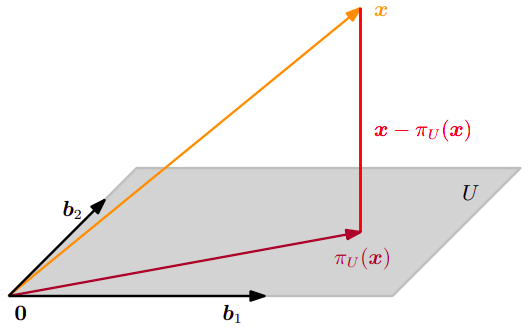
\includegraphics[
        width=\linewidth,
        height=4cm,
        keepaspectratio,
    ]{images/maths-for-ml/Projection-2d.png}
    \caption*{
        Projection onto a two-dimensional subspace $U$ with basis $\bm{b}_1$, $\bm{b}_2$. 
        The projection $\pi_U (\bm{x})$ of $\bm{x} \in \mathbb{R}^3$ onto $U$ can be expressed as a linear combination of $\bm{b}_1, \bm{b}_2$ and the displacement vector $\bm{x} - \pi_U (\bm{x})$ is orthogonal to both $\bm{b}_1$ and $\bm{b}_2$.
        \cite{mfml/book/mml/Deisenroth-Faisal-Ong}
    }
\end{figure}


\begin{enumerate}
    \item orthogonal projections of vectors $\bm{x} \in \mathbb{R}^n$ onto lower-dimensional subspaces $U \subseteq \mathbb{R}^n$ with $\dim(U) = m \geq 1$.

    \item Assume that $(\bm{b}_1, \cdots , \bm{b}_m)$ is an ordered basis of $U$.
    If $U$ is given by a set of spanning vectors, which are not a basis, make sure you determine a basis $\bm{b}_1, \cdots , \bm{b}_m$ before proceeding.

    \item Steps:
    \begin{enumerate}
        \item Find the coordinates $\lambda_1, \cdots , \lambda_m$ of the projection (with respect to the basis of $U$), such that the linear combination:
        \hfill \cite{mfml/book/mml/Deisenroth-Faisal-Ong}
        \\
        .\hfill
        $
            \pi_U (\bm{x}) = \dsum^m _{i=1} \lambda_i \bm{b}_i = \bm{B \lambda}
        $
        \hfill \cite{mfml/book/mml/Deisenroth-Faisal-Ong}
        \\
        .\hfill
        $
            \bm{B} = [\bm{b}_1, \cdots , \bm{b}_m] \in \mathbb{R}^{n\times m}, 
            \bm{\lambda} = [\lambda_1, \cdots , \lambda_m]^\top \in \mathbb{R}^m
        $
        \hfill \cite{mfml/book/mml/Deisenroth-Faisal-Ong}
        \\[0.2cm]
        is closest to $\bm{x} \in \mathbb{R}^n$.
        “Closest” means “minimum distance”, which implies that the vector connecting $\pi_U (\bm{x}) \in U$ and $\bm{x} \in \mathbb{R}^n$ must be orthogonal to all basis vectors of $U$.
        \hfill \cite{mfml/book/mml/Deisenroth-Faisal-Ong}
        \\
        we obtain $m$ simultaneous conditions (assuming the dot product as the inner product)
        \\
        .\hfill
        $
            \begin{aligned}
                \dAngleBrac{\bm{b}_1, \bm{x} - \pi _U (\bm{x})} 
                    &= \bm{b} ^\top _1 (\bm{x} - \pi _U (\bm{x})) = 0 
                \\
                & \vdots 
                \\
                \dAngleBrac{\bm{b}_m, \bm{x} - \pi _U (\bm{x})} 
                    &= \bm{b} ^\top _m(\bm{x} - \pi _U (\bm{x})) = 0
            \end{aligned}
        $
        \hfill \cite{mfml/book/mml/Deisenroth-Faisal-Ong}
        \\
        which, with $\pi_U (\bm{x}) = \bm{B \lambda}$, can be written as
        \hfill \cite{mfml/book/mml/Deisenroth-Faisal-Ong}
        \\[0.2cm]
        .\hfill
        $
            \bm{b}^\top _1(\bm{x} - \bm{B \lambda}) = 0
            \hspace{1cm}
            \cdots
            \hspace{1cm}
            \bm{b}^\top _m(\bm{x} - \bm{B \lambda}) = 0
        $
        \hfill \cite{mfml/book/mml/Deisenroth-Faisal-Ong}
        \\
        such that we obtain a homogeneous linear equation system
        \hfill \cite{mfml/book/mml/Deisenroth-Faisal-Ong}
        \\
        .\hfill
        $
                \begin{bmatrix}
                    \bm{b}^\top _1 \\
                    \vdots \\
                    \bm{b}^\top _m
                \end{bmatrix}
                \begin{bmatrix}
                    \\
                    \bm{x} - \bm{B\lambda} \\
                    \\
                \end{bmatrix} = \bm{0}
                \hspace{0.5cm}
                \Longleftrightarrow
                \hspace{0.5cm}
                \bm{B}^\top (\bm{x} - \bm{B\lambda}) = \bm{0} 
                \hspace{0.5cm}
                \Longleftrightarrow
                \hspace{0.5cm}
                \bm{B}^\top \bm{B\lambda} = \bm{B}^\top \bm{x}
        $
        \hfill \cite{mfml/book/mml/Deisenroth-Faisal-Ong}
        \\
        $\bm{B}^\top \bm{B\lambda} = \bm{B}^\top \bm{x}$ is called \textbf{normal equation}.
        Since $\bm{b}_1, \cdots , \bm{b}_m$ are a basis of $U$ and, therefore, linearly independent, $\bm{B}^\top \bm{B} \in \mathbb{R}^{m\times m}$ is regular and can be inverted. 
        \hfill \cite{mfml/book/mml/Deisenroth-Faisal-Ong}
        \\
        .\hfill
        $
            \bm{\lambda} = (\bm{B}^\top \bm{B})^{-1} \bm{B}^\top \bm{x}
        $
        \hfill \cite{mfml/book/mml/Deisenroth-Faisal-Ong}
        \\
        $(\bm{B}^\top \bm{B})^{-1} \bm{B}^\top$ is also called the pseudo-inverse of $\bm{B}$
        \hfill \cite{mfml/book/mml/Deisenroth-Faisal-Ong}
        \\
        In practical applications (e.g., linear regression), we often add a “\textbf{jitter term}” $\epsilon \bm{I}$ to $\bm{B}^\top \bm{B}$ to guarantee increased numerical stability and positive definiteness. 
        This “ridge” can be rigorously derived using Bayesian inference. 
        \hfill \cite{mfml/book/mml/Deisenroth-Faisal-Ong}
        \\
        A ridge term is essentially the same as a jitter term but used in the context of regularization, especially in ridge regression (also called Tikhonov regularization). 
        \hfill \cite{common/online/chatgpt}

        \item Find the projection $\pi_U (\bm{x}) \in U$:
        \hfill \cite{mfml/book/mml/Deisenroth-Faisal-Ong}
        \\
        .\hfill
        $
            \pi_U (\bm{x}) 
            = \bm{B\lambda}
            = \bm{B} (\bm{B}^\top \bm{B})^{-1} \bm{B}^\top \bm{x}
        $
        \hfill \cite{mfml/book/mml/Deisenroth-Faisal-Ong}

        \item Find the projection matrix $\bm{P} _\pi$:
        \hfill \cite{mfml/book/mml/Deisenroth-Faisal-Ong}
        \\
        .\hfill
        $
            \pi_U (\bm{x}) = \bm{P} _\pi \bm{x} = \bm{B} (\bm{B}^\top \bm{B})^{-1} \bm{B}^\top \bm{x}
            \hspace{0.5cm}
            \Longleftrightarrow
            \hspace{0.5cm}
            \bm{P} _\pi 
                = \bm{B} (\bm{B}^\top \bm{B})^{-1} \bm{B}^\top
                = \dfrac{\bm{B}\bm{B}^\top}{\bm{B}^\top \bm{B}}
        $
        \hfill \cite{mfml/book/mml/Deisenroth-Faisal-Ong}
    \end{enumerate}
\end{enumerate}




\begin{lstlisting}[
    language=Python,
    caption=Projection onto General Subspaces - numPy
]
import numpy as np

def project_onto_subspace(x, B):
    """
    Projects vector x onto the subspace spanned by the column vectors of matrix B.

    Args:
        x: A numpy array of shape (n,) representing the vector to project
        B: A numpy array of shape (n, m) whose 
            columns are basis vectors of the subspace

    Returns:
        lambda_vec: Coordinate vector lambda such that projection = B @ lambda_vec
        projection: The projection vector of x onto the subspace spanned by B
        projection_matrix: The projection matrix P such that P @ x = projection
    """
    # Reshape x as column vector
    x = x.reshape(-1, 1)

    # Compute (B^T B)^(-1) B^T x
    BtB_inv = np.linalg.inv(B.T @ B)
    lambda_vec = BtB_inv @ B.T @ x

    # Compute projection: B @ lambda
    projection = B @ lambda_vec

    # Projection matrix: B (B^T B)^(-1) B^T
    projection_matrix = B @ BtB_inv @ B.T

    return lambda_vec, projection, projection_matrix

# Example usage
x = np.array([2, 3, 4])

# Define individual basis vectors (as 1D arrays or column vectors)
b1 = np.array([1, 0, 1])
b2 = np.array([0, 1, 1])

# Stack them as columns to form matrix B
B = np.column_stack((b1, b2))  # Equivalent to np.stack((b1, b2), axis=1)

lambda_vec, projection_vec, projection_mat = project_onto_subspace(x, B)

print("Coordinate vector lambda:\n", lambda_vec)
print("Projection vector:\n", projection_vec)
print("Projection matrix:\n", projection_mat)

# should equal projection_vec
print("P @ x:\n", projection_mat @ x.reshape(-1, 1))  
\end{lstlisting}

output:
\begin{lstlisting}[
    % language=Python,
    % caption=Projection onto One-Dimensional Subspaces (Lines) - numPy
]
Coordinate vector lambda:
 [[1.66666667]
 [2.66666667]]
Projection vector:
 [[1.66666667]
 [2.66666667]
 [4.33333333]]
Projection matrix:
 [[ 0.66666667 -0.33333333  0.33333333]
 [-0.33333333  0.66666667  0.33333333]
 [ 0.33333333  0.33333333  0.66666667]]
P @ x:
 [[1.66666667]
 [2.66666667]
 [4.33333333]]
\end{lstlisting}









\subsection{Projection onto Affine Subspaces}

\begin{figure}[H]
    \centering
    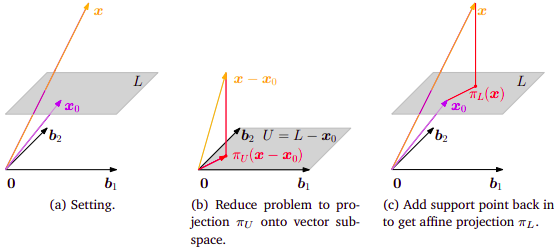
\includegraphics[
        width=\linewidth,
        height=5cm,
        keepaspectratio,
    ]{images/maths-for-ml/Projection-onto-Affine-Subspaces.png}
    \caption*{
        Projection onto an affine space.
        \\
        (a) original setting; 
        \hfill \cite{mfml/book/mml/Deisenroth-Faisal-Ong}
        \\
        (b) setting shifted by $-\bm{x}_0$ so that $\bm{x} - \bm{x}_0$ can be projected onto the direction space $U$;
        \hfill \cite{mfml/book/mml/Deisenroth-Faisal-Ong}
        \\
        (c) projection is translated back to $\bm{x}_0 + \pi_U (\bm{x} - \bm{x}_0)$, which gives the final orthogonal projection $\pi_L(\bm{x})$.
        \hfill \cite{mfml/book/mml/Deisenroth-Faisal-Ong}
    }
\end{figure}


\begin{enumerate}
    \item We are given an affine space $L = \bm{x}_0 + U$, where $\bm{b}_1$, $\bm{b}_2$ are basis vectors of $U$.
    \hfill \cite{mfml/book/mml/Deisenroth-Faisal-Ong}

    \item To determine the orthogonal projection $\pi_L(\bm{x})$ of $\bm{x}$ onto $L$, we transform the problem into a problem that we know how to solve: the projection onto a vector subspace.
    \hfill \cite{mfml/book/mml/Deisenroth-Faisal-Ong}

    \item  In order to get there, we subtract the support point $\bm{x}_0$ from $\bm{x}$ and from $L$, so that $L - \bm{x}_0 = U$ is exactly the vector subspace $U$. 
    \hfill \cite{mfml/book/mml/Deisenroth-Faisal-Ong}
    
    \item We can now use the orthogonal projections onto a subspace and obtain the projection $\pi_U (\bm{x} - \bm{x}_0)$.
    \hfill \cite{mfml/book/mml/Deisenroth-Faisal-Ong}

    \item This projection can now be translated back into $L$ by adding $\bm{x}_0$, such that we obtain the orthogonal projection onto an affine space $L$ as:
    \hfill \cite{mfml/book/mml/Deisenroth-Faisal-Ong}
    \\
    .\hfill
    $
        \pi_L(\bm{x}) = \bm{x}_0 + \pi_U (\bm{x} - \bm{x}_0)
    $
    \hfill \cite{mfml/book/mml/Deisenroth-Faisal-Ong}
    \\
    where $\pi_U (\cdot)$ is the orthogonal projection onto the subspace $U$, i.e., the direction space of $L$.
    \hfill \cite{mfml/book/mml/Deisenroth-Faisal-Ong}

    \item it is also evident that the distance of $\bm{x}$ from the affine space $L$ is identical to the distance of $\bm{x} - \bm{x}_0$ from $U$, i.e.,
    \hfill \cite{mfml/book/mml/Deisenroth-Faisal-Ong}
    \\
    .\hfill
    $
        d(\bm{x}, L) 
        = \dnorm{\bm{x} - \pi_L(x)} 
        = \dnorm{\bm{x} - (\bm{x}_0 + \pi_U (\bm{x} - \bm{x}_0))}
        = d(\bm{x} - \bm{x}_0, \pi_U (\bm{x} - \bm{x}_0)) 
        = d(\bm{x} - \bm{x}_0, U)
    $
    \hfill \cite{mfml/book/mml/Deisenroth-Faisal-Ong}
\end{enumerate}




\section{Rotations ($\Phi$) \& Rotation Matrix ($R(\theta)$)}



\begin{enumerate}
    \item A rotation is a linear mapping (more specifically, an automorphism of rotation a Euclidean vector space) that rotates a plane by an angle $\theta$ about the origin, i.e., the origin is a fixed point.
    \hfill \cite{mfml/book/mml/Deisenroth-Faisal-Ong}
    
    \item For a positive angle $\theta > 0$, by common convention, we rotate in a counterclockwise direction.
    \hfill \cite{mfml/book/mml/Deisenroth-Faisal-Ong}

    \item The rotated vectors are still linearly independent and, therefore, are a basis of $\mathbb{R}^2$. 
    This means that the rotation performs a basis change.
    \hfill \cite{mfml/book/mml/Deisenroth-Faisal-Ong}

    \item Rotations $\Phi$ are linear mappings so that we can express them by a rotation matrix $\bm{R}(\theta)$. 
    \hfill \cite{mfml/book/mml/Deisenroth-Faisal-Ong}

    \item \textbf{Properties}:
    \begin{enumerate}
        \item Rotations preserve distances, i.e., $\dnorm{\bm{x}-\bm{y}} = \dnorm{\bm{R}_\theta (\bm{x}) - \bm{R}_\theta (\bm{y})}$. In other words, rotations leave the distance between any two points unchanged after the transformation.
        \hfill \cite{mfml/book/mml/Deisenroth-Faisal-Ong}

        \item Rotations preserve angles, i.e., the angle between $\bm{R}_\theta \bm{x}$ and $\bm{R}_\theta \bm{y}$ equals the angle between $\bm{x}$ and $\bm{y}$.
        \hfill \cite{mfml/book/mml/Deisenroth-Faisal-Ong}

        \item Rotations in three (or more) dimensions are generally not commutative. 
        Therefore, the order in which rotations are applied is important, even if they rotate about the same point. 
        \hfill \cite{mfml/book/mml/Deisenroth-Faisal-Ong}
        
        \item Only in two dimensions vector rotations are commutative, such that $\bm{R}(\phi)\bm{R}(\theta ) = \bm{R}(\theta )\bm{R}(\phi) \hspace{0.2cm} \forall \phi, \theta  \in [0, 2\pi)$. 
        They form an Abelian group (with multiplication) only if they rotate about the same point (e.g., the origin).
        \hfill \cite{mfml/book/mml/Deisenroth-Faisal-Ong}
    \end{enumerate}
\end{enumerate}


\subsection{Rotations in $R^2$}


\begin{figure}[H]
    \centering
    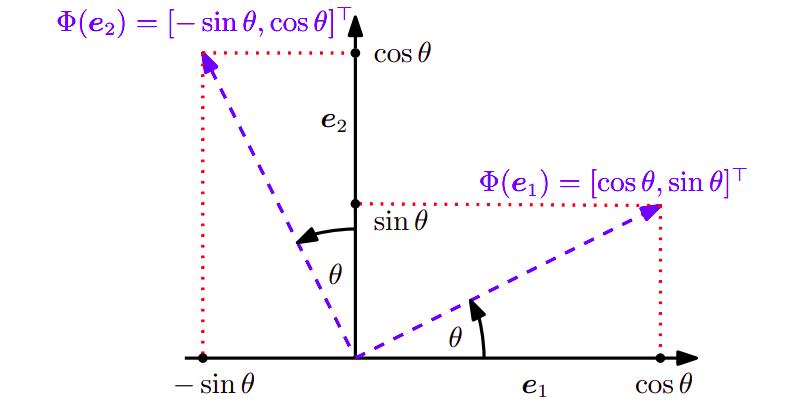
\includegraphics[
        width=\linewidth,
        height=4cm,
        keepaspectratio,
    ]{images/maths-for-ml/rotations-r2.png}
    \caption{
        Rotation of the standard basis in $\mathbb{R}^2$ by an angle $\theta$.
        \cite{mfml/book/mml/Deisenroth-Faisal-Ong}
    }
\end{figure}


\begin{enumerate}
    \item Consider the standard basis 
    $
        \dCurlyBrac{
            \bm{e}_1 = \begin{bmatrix}1\\0\end{bmatrix}, 
            \bm{e}_2 = \begin{bmatrix}0\\1\end{bmatrix}
        }
    $ of $\mathbb{R}^2$ , which defines the standard coordinate system in $\mathbb{R}^2$.
    \hfill \cite{mfml/book/mml/Deisenroth-Faisal-Ong}

    \item using trigonometry:
    $
        \Phi(\bm{e}_1) = \begin{bmatrix}\cos \theta\\\sin \theta\end{bmatrix},
        \hspace{0.15cm}
        \Phi(\bm{e}_2) = \begin{bmatrix}-\sin \theta\\\cos \theta\end{bmatrix}
    $
    \hfill \cite{mfml/book/mml/Deisenroth-Faisal-Ong}

    \item the rotation matrix that performs the basis change into the rotated coordinates $\bm{R}(\theta)$ is given as:
    \hfill \cite{mfml/book/mml/Deisenroth-Faisal-Ong}
    \\
    .\hfill
    $
        \bm{R}(\theta)
        = \begin{bmatrix}
            \Phi(\bm{e}_1) & \Phi(\bm{e}_2)
        \end{bmatrix}
        = \begin{bmatrix}
            \cos\theta & -\sin\theta \\
            \sin\theta & \cos\theta
        \end{bmatrix}
    $
    \hfill \cite{mfml/book/mml/Deisenroth-Faisal-Ong}
\end{enumerate}


\subsection{Rotations in $R^3$}


\begin{figure}[H]
    \centering
    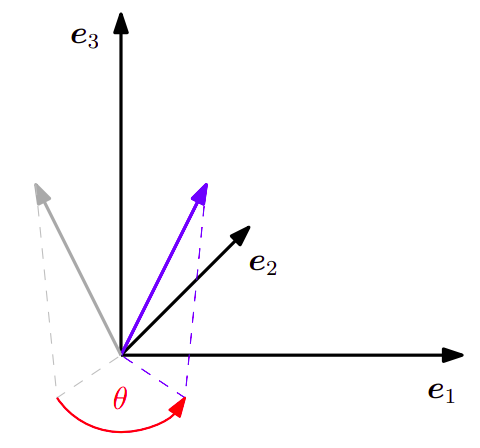
\includegraphics[
        width=\linewidth,
        height=4cm,
        keepaspectratio,
    ]{images/maths-for-ml/rotations-r3.png}
    \caption{
        Rotation of a vector (gray) in $\mathbb{R}^3$ by an angle $\theta$ about the $\bm{e}_3$-axis. 
        The rotated vector is shown in blue.
        \cite{mfml/book/mml/Deisenroth-Faisal-Ong}
    }
\end{figure}

\begin{enumerate}
    \item In contrast to the $\mathbb{R}^2$ case, in $\mathbb{R}^3$ we can rotate any two-dimensional plane about a one-dimensional axis.
    \hfill \cite{mfml/book/mml/Deisenroth-Faisal-Ong}

    \item The easiest way to specify the general rotation matrix is to specify how the images of the standard basis $\bm{e}_1$, $\bm{e}_2$, $\bm{e}_3$ are supposed to be rotated, and making sure these images $\bm{Re}_1$, $\bm{Re}_2$, $\bm{Re}_3$ are orthonormal to each other. 
    We can then obtain a general rotation matrix $\bm{R}$ by combining the images of the standard basis.
    \hfill \cite{mfml/book/mml/Deisenroth-Faisal-Ong}

    \item We use the convention that a “counterclockwise” (planar) rotation about an axis refers to a rotation about an axis when we look at the axis “head on, from the end toward the origin”.
    \hfill \cite{mfml/book/mml/Deisenroth-Faisal-Ong}



    \item Rotation about the $\bm{e}_1$-axis:
    \hfill \cite{mfml/book/mml/Deisenroth-Faisal-Ong}
    \\
    .\hfill
    $
        \bm{R}_1(\theta) 
        = \begin{bmatrix}\Phi(\bm{e}_1) & \Phi(\bm{e}_2) & \Phi(\bm{e}_3)\end{bmatrix}
        = \begin{bmatrix}
        1 & 0 & 0 \\
        0 & \cos \theta & - \sin \theta \\
        0 & \sin \theta & \cos \theta \\
        \end{bmatrix}
    $
    \hfill \cite{mfml/book/mml/Deisenroth-Faisal-Ong}
    \\
    Here, the $\bm{e}_1$ coordinate is fixed, and the counterclockwise rotation is performed in the $\bm{e}_2\bm{e}_3$ plane.
    \hfill \cite{mfml/book/mml/Deisenroth-Faisal-Ong}



    \item Rotation about the $\bm{e}_2$-axis:
    \hfill \cite{mfml/book/mml/Deisenroth-Faisal-Ong}
    \\
    .\hfill
    $
        \bm{R}_2(\theta) 
        = \begin{bmatrix}
        \cos \theta & 0 &  \sin \theta \\
        0 & 1 & 0 \\
        - \sin \theta & 0 & \cos \theta \\
        \end{bmatrix}
    $
    \hfill \cite{mfml/book/mml/Deisenroth-Faisal-Ong}
    \\
    If we rotate the $\bm{e}_1\bm{e}_3$ plane about the $\bm{e}_2$ axis, we need to look at the $\bm{e}_2$ axis from its “tip” toward the origin.
    \hfill \cite{mfml/book/mml/Deisenroth-Faisal-Ong}



    \item Rotation about the $\bm{e}_3$-axis:
    \hfill \cite{mfml/book/mml/Deisenroth-Faisal-Ong}
    \\
    .\hfill
    $
        \bm{R}_3(\theta) 
        = \begin{bmatrix}
        \cos \theta &   -\sin \theta & 0\\
        \sin \theta &  \cos \theta & 0\\
        0 & 0 & 1 \\
        \end{bmatrix}
    $
    \hfill \cite{mfml/book/mml/Deisenroth-Faisal-Ong}
    
\end{enumerate}


\subsection{Rotations in $n$ Dimensions (Givens Rotation)}

\begin{enumerate}
    \item The generalization of rotations from $2$D and $3$D to $n$-dimensional Euclidean vector spaces can be intuitively described as fixing $n - 2$ dimensions and restrict the rotation to a two-dimensional plane in the $n$-dimensional space.

    \item
    \begin{definition}[Givens Rotation]
        Let $V$ be an $n$-dimensional Euclidean vector space and $\Phi : V \to V$ an automorphism with transformation matrix:
        \\
        .\hfill
        $
            \bm{R}_{ij} (\theta) := 
            \begin{bmatrix}
                \bm{I}_{i-1} & 0 & \cdots &  \cdots & 0 \\
                0 & \cos \theta & 0 & - \sin \theta & 0\\
                0 & 0 & \bm{I}_{j-i-1} & 0 & 0\\
                0 & \sin \theta &  0 & \cos \theta & 0\\
                0 & \cdots & \cdots & 0 & \bm{I}_{n-j}
            \end{bmatrix}
            \in \mathbb{R}^{n\times n}
        $
        \hfill \cite{mfml/book/mml/Deisenroth-Faisal-Ong}
        \\
        for $1 \leq i < j \leq n$ and $\theta \in \mathbb{R}$. 
        Then $\bm{R}_{ij} (\theta)$ is called a Givens rotation. 
        Essentially, $\bm{R}_{ij} (\theta)$ is the identity matrix $\bm{I}_n$ with
        \hfill \cite{mfml/book/mml/Deisenroth-Faisal-Ong}
        \\
        .\hfill
        $
            r_{ii} = \cos \theta , 
            \hspace{0.2cm}
            r_{ij} = - \sin \theta,
            \hspace{0.2cm}
            r_{ji} = \sin \theta, 
            \hspace{0.2cm}
            r_{jj} = \cos \theta
        $
        \hfill \cite{mfml/book/mml/Deisenroth-Faisal-Ong}
    \end{definition}

    \item \textbf{Note}: 2D is special case
\end{enumerate}





























